% ================================================================
% Do Post-Training Algorithms Actually Differ?
% Target: NeurIPS 2026 — Camera-Ready (9 pages)
% ================================================================
\documentclass{article}

% NeurIPS 2026 style
\usepackage[eandd]{neurips_2026}

% Packages
\usepackage[utf8]{inputenc}
\usepackage[T1]{fontenc}
\usepackage{hyperref}
\usepackage{url}
\usepackage{booktabs}
\usepackage{amsfonts}
\usepackage{amsmath}
\usepackage{amssymb}
\usepackage{nicefrac}
\usepackage{microtype}
\usepackage{graphicx}
\graphicspath{{figures/}}
\usepackage{xcolor}
\usepackage{subcaption}
\usepackage{multirow}
\usepackage{enumitem}
\usepackage{algorithm}
\usepackage{algorithmic}

% Custom commands
\newcommand{\ours}{\textsc{oxRL}}
\newcommand{\sprft}{SP-RFT}

\title{Do Post-Training Algorithms Actually Differ\\ on Mathematical Reasoning at Scale?}

\author{
  Anonymous Authors
}

\begin{document}

\maketitle

% ================================================================
% ABSTRACT
% ================================================================
\begin{abstract}
Practitioners routinely benchmark post-training algorithms---DPO, SimPO, KTO, GRPO, and dozens of variants---at small scale, then deploy the winner at large scale.
We show this practice is \emph{anti-predictive} for mathematical reasoning: algorithm rankings invert as models grow.
In a controlled study spanning ${\sim}$350 training runs across two model families (Qwen~2.5 0.5B--14B, Gemma~3 1B--12B), 8 algorithms, 20 DPO variants, and up to $N{=}5$ seeds---using model-specific self-play data matching standard practitioner workflows---we find three results that challenge common intuitions.
Importantly, these effects are task-specific: on multiple-choice general benchmarks (ARC-C, HellaSwag, WinoGrande), algorithms differ by $<$1.2~pp at all scales, and no inversion is observable---though generative instruction-following evaluations remain untested.
\textbf{(1)~Rankings invert with scale (from Instruct checkpoints).} At $\leq$1.5B, Self-Play RFT (\sprft{})---which trains on the model's own correct trajectories, functionally rejection sampling fine-tuning~\citep{yuan2023rft}---is the strongest offline method; at 7B, \sprft{} collapses to worst while DPO leads ($p < 0.001$, $N{=}5$). A gold-data control confirms this is not an RFT artifact: standard SFT on MetaMathQA also dominates at 1.5B but converges to DPO at 7B. The same inversion appears in Gemma~3 (1B--12B) and persists at Qwen~14B (DPO leads \sprft{} by 2.2~pp), though the within-family gap narrows from 6.0~pp at 7B. We also evaluated 20 DPO variants; under shared default hyperparameters ($\beta{=}0.1$, LR${=}10^{-6}$), their point-estimate rankings reverse but are statistically unresolvable, highlighting that variant sweeps require per-variant tuning at target scale (Appendix~\ref{app:dpo_full}).
\textbf{(2)~Initialization dominates algorithm choice.} Replacing the Instruct checkpoint with Base collapses the inter-algorithm accuracy spread from 15.7~pp to 1.07~pp at 1.5B and from 6.00~pp to 1.82~pp at 7B (a 3--15$\times$ compression). A residual ranking shift persists from Base, but at $\leq$1.8~pp---revealing that most observed differences arise from the interaction between loss functions and prior alignment.
\textbf{(3)~Apparent differences have two regimes.} At small scale ($\leq$1.5B), the 19.3~pp GSM8K spread collapses $36\times$ to 0.54~pp on MATH---the GSM8K inversion is largely a format-compliance-to-reasoning shift, as MATH scores begin effectively tied. At large scale ($\geq$4B), MATH reveals genuine reasoning differences, but these are \emph{architecture-dependent}: DPO dominates Gemma MATH by +9~pp while SimPO dominates Qwen~14B MATH by +13~pp. Rankings cannot be extrapolated across scales, architectures, or tasks.
A fixed-dataset control confirms that the inversion is scale-driven, not a data-quality artifact. A gold-data control rules out the hypothesis that the inversion is an artifact of self-play RFT.
Together, these findings imply that small-scale algorithm selection---the dominant paradigm in both research and practice---is unreliable for mathematical reasoning, and that practitioners should validate at deployment scale, on their target architecture and task, rather than extrapolating from cheap proxies. Whether these inversions extend to other post-training objectives (instruction following, safety, creative writing) remains an open question.
\end{abstract}

% ================================================================
% 1. INTRODUCTION
% ================================================================
\section{Introduction}

Suppose you are choosing a post-training algorithm for mathematical reasoning. You benchmark Self-Play RFT (\sprft{}), DPO, and SimPO at 1.5B parameters: \sprft{} wins by 5~pp over DPO. You select \sprft{}, scale to 7B, and deploy---only to discover that \sprft{} is now the \emph{worst} method by 6~pp, while DPO has silently become best. Your small-scale selection was not just uninformative; it was anti-predictive.

This is not a hypothetical. It is the central empirical finding of this paper, replicated across two model families and confirmed with formal statistical testing ($p < 0.001$, $N{=}5$ seeds). The practitioner's dilemma is real: every published comparison operates at a single scale, yet deployment happens at a different one. If rankings invert, the entire methodology of algorithm benchmarking at small scale is called into question.

Post-training of large language models---adapting a pretrained model for tasks such as mathematical reasoning---has become the decisive stage separating a capable base model from a useful one~\citep{ouyang2022training, touvron2023llama2}. Many algorithms compete for adoption: online RL methods like GRPO~\citep{shao2024deepseekmath}, offline preference methods like DPO~\citep{rafailov2023direct}, and a growing family of variants---SimPO~\citep{meng2024simpo}, KTO~\citep{ethayarajh2024kto}, ORPO~\citep{hong2024orpo}---each claiming improvements over prior work. DeepSeek-R1~\citep{deepseek2025r1} demonstrated that pure RL post-training can elicit sophisticated reasoning, further expanding the design space. Yet each paper evaluates on different models, datasets, and scales, making cross-method comparison unreliable. The few existing studies~\citep{xu2024dpo, spangher2025rlhf} cover limited methods at a single scale---they cannot detect the ranking inversions we observe.

We address this gap through a large-scale, controlled comparison using a unified framework where all algorithms share identical infrastructure. Our thesis is sharp: \textbf{on mathematical reasoning, post-training algorithm rankings invert with scale, making small-scale selection anti-predictive.} We emphasize that this is a task-specific phenomenon: on multiple-choice general benchmarks (ARC-C, HellaSwag, WinoGrande), algorithms differ by $<$1.2~pp at all scales (Section~\ref{sec:format_compliance}; Appendix~\ref{app:general_benchmarks}), though generative benchmarks remain untested. The evidence for mathematical reasoning unfolds in three findings:

\begin{enumerate}[leftmargin=*,itemsep=2pt]
    \item \textbf{Rankings invert with scale---from Instruct checkpoints, across architectures.}
    On Qwen~2.5 Instruct, \sprft{} leads offline methods at $\leq$3B but collapses to worst at 7B, where DPO (83.4\%~$\pm$0.56) and SimPO (83.3\%~$\pm$1.79) dominate ($p < 0.001$ vs.\ \sprft{}, $N{=}5$). On Gemma~3 IT, the same pattern holds: \sprft{}~$>$~DPO at 1B and 4B, but DPO~$\geq$~\sprft{} at 12B (87.4\% vs.\ 86.7\%).

    \item \textbf{Initialization explains most of the variance.}
    Replacing Instruct with Base initialization collapses the inter-algorithm spread from 15.7~pp to 1.07~pp at 1.5B and from 6.00~pp to 1.82~pp at 7B (a 3--15$\times$ compression). The dominant source of inter-algorithm variance is how each loss function interacts with prior alignment, not intrinsic properties of the objectives.

    \item \textbf{Apparent differences have two regimes: format compliance at small scale, architecture-specific reasoning at large scale.}
    At 1.5B, the 19.3~pp GSM8K spread collapses $36\times$ to 0.54~pp on MATH and $41\times$ to 0.47~pp on general benchmarks---algorithms differ only in format compliance. At larger scales ($\geq$4B), MATH reveals genuine reasoning differences, but these depend on the (algorithm, architecture) pair: DPO gains +9~pp on Gemma~12B MATH while SimPO gains +13~pp on Qwen~14B MATH. Both regimes yield the same practical conclusion: small-scale benchmarking is unreliable.
\end{enumerate}

These findings are based on ${\sim}$323 training runs on Qwen~2.5 (0.5B--14B), supplemented by 27 runs on Gemma~3 (1B--12B), spanning 8 algorithms, 20 DPO variants, 4 evaluation domains (GSM8K, MATH, ARC-C/HellaSwag/WinoGrande), and up to $N{=}5$ seeds with formal statistical testing.
The implication for practitioners is direct: validate at deployment scale, not prototype scale. The implication for the research community is that designing new loss functions at small scale---the dominant paradigm---may be selecting for the wrong properties.

% ================================================================
% 2. RELATED WORK
% ================================================================
\section{Related Work}

\textbf{Post-training algorithms and comparative studies.}
The RLHF pipeline~\citep{ouyang2022training} uses PPO~\citep{schulman2017proximal}; GRPO~\citep{shao2024deepseekmath} simplifies this via group-normalized rewards.
\citet{wu2025grpo_dpo} show theoretical equivalence between GRPO and DPO; our empirical results reveal an 8.9~pp gap in practice.
DPO~\citep{rafailov2023direct} bypasses reward modeling, spawning IPO~\citep{azar2024general}, SimPO~\citep{meng2024simpo}, KTO~\citep{ethayarajh2024kto}, ORPO~\citep{hong2024orpo}, and others.
We provide the first controlled evaluation of 20 DPO variants under identical conditions.
\citet{xu2024dpo} and \citet{ivison2024unpacking} cover only 2--3 algorithms.
\citet{spangher2025rlhf} benchmark 17 algorithms at a single scale---they cannot detect ranking inversions.
\citet{saeidi2025dpo_variants} evaluate DPO variants without multi-seed runs or multiple comparison correction.
Our finding that variant rankings are scale-dependent is reminiscent of \citet{lucic2018gans}, who found that GAN variant rankings change across experimental conditions.
Critically, none of these studies evaluate across multiple model families, leaving the question of architectural generality unanswered. Our Gemma~3 validation addresses this gap.
\citet{tan2025rl_scaling} study scaling behaviors of RL post-training; our work complements theirs by showing that \emph{relative} rankings---not just absolute performance---are scale-dependent.

% ================================================================
% 3. METHODS AND EXPERIMENTAL SETUP
% ================================================================
\section{Methods and Experimental Setup}
\label{sec:methods}

\label{sec:framework}

\textbf{Framework.} Our framework provides a single codebase where all 51 algorithms share identical model loading (HuggingFace, \texttt{flash\_attention\_2}), data pipelines, distributed training (DeepSpeed ZeRO-3~\citep{rajbhandari2020zero}, vLLM~\citep{kwon2023efficient} for RL rollouts), and checkpointing. Each algorithm implements a \texttt{BaseAlgorithm} interface requiring only the loss function, ensuring the \emph{only} difference between runs is the loss computation. We organize algorithms into: \textbf{(1)~\sprft{};} \textbf{(2)~Online RL} (GRPO variants); \textbf{(3)~Offline preference} (DPO~\citep{rafailov2023direct}, IPO~\citep{azar2024general}, SimPO~\citep{meng2024simpo}, KTO~\citep{ethayarajh2024kto}, and 16 additional variants); \textbf{(4)~Hybrid} (ORPO~\citep{hong2024orpo}, SPIN~\citep{chen2024spin}). The 20-variant taxonomy is in Appendix~\ref{app:dpo_full}.

\textbf{Evaluation.} GSM8K~\citep{cobbe2021gsm8k} (1,319 test problems, exact-match, greedy decoding). MATH~\citep{hendrycks2021math} (5,000 problems, 4-shot) at 1.5B and general-domain benchmarks (ARC-C, HellaSwag, WinoGrande) at both 1.5B and 7B. All evaluations use the LM Evaluation Harness~\citep{eval-harness}. We report means $\pm \sigma$ and perform Welch's $t$-tests with Bonferroni correction where indicated.

\label{sec:eval_protocol}
\label{sec:setup}

\textbf{Qwen 2.5 (primary).} Qwen 2.5~\citep{qwen2025qwen25} Instruct at 0.5B, 1.5B, 3B, 7B, and 14B. Our experiments comprise: (1) core comparison of 8 algorithms across 4 scales ($\sim$70 runs, $N{=}5$ seeds for core methods at 7B), with a full-FT/LoRA factorial at both 3B and 7B; (2) DPO variant taxonomy at 1.5B (20 variants $\times$ 5 seeds = 100 runs) and a stratified subset of 5 at 7B (15 runs); (3) 14B deployment-scale validation with \sprft{}, DPO, SimPO ($N{=}3$ seeds each); (4) ablations ($\sim$57 runs), including Base-vs-Instruct initialization and hyperparameter sensitivity; (5) a fixed-dataset control training 1.5B on 14B self-play data (6 runs, Section~\ref{sec:controls}); (6) LR sweeps at 1.5B, 3B, and 7B (54 runs, Appendix~\ref{app:lr_ablation}--\ref{app:lr_ablation_3b}); (7) a gold-data SFT control using MetaMathQA at 1.5B and 7B (6 runs, Section~\ref{sec:controls}). Total: $\sim$323 training runs, $\sim$740 GPU-hours on H100s (Appendix~\ref{app:compute}).

\textbf{Gemma 3 (cross-architecture validation).} To test whether our findings generalize beyond Qwen, we train \sprft{}, DPO, and SimPO on Gemma~3~\citep{gemma3_2025} IT at 1B, 4B, and 12B with 3 seeds each (27 runs). This uses the same GSM8K data and evaluation protocol; 12B uses LoRA, matching the Qwen 7B setup.

\textbf{Data.} All algorithms share the same data pipeline to eliminate data-source confounds. For each prompt in GSM8K's 7,473 training problems, we sample 16 responses from the \emph{target model} at temperature 1.0 and score each with exact-match correctness. DPO/SimPO/IPO receive (chosen, rejected) pairs from the highest/lowest scoring responses. \sprft{} trains on the \emph{chosen} trajectories from this same self-play dataset---not gold responses---ensuring that only the loss function differs between methods. Because \sprft{} trains on model-generated chosen trajectories rather than gold or expert data, it is functionally \emph{rejection sampling fine-tuning} (RFT)~\citep{yuan2023rft}; we use the \sprft{} label to distinguish it from standard SFT on gold data (Section~\ref{sec:controls}). This distinction matters mechanistically: at small scale, where few model samples are correct, RFT on rare successes yields large gains; at large scale, where the model already solves most problems, RFT encounters a ceiling effect while DPO's contrastive signal can still extract improvements (see Section~\ref{sec:discussion}).

\textbf{Design rationale.} Data is generated \emph{at each scale}, matching how practitioners train~\citep{shao2024deepseekmath, deepseek2025r1, chen2024spin}. Dataset quality therefore correlates with model scale; we address this confound with a fixed-dataset control (Section~\ref{sec:controls}).
\textbf{Training.} AdamW, cosine LR ($10^{-6}$) with 10\% warmup, 3 epochs, batch size 8. LoRA~\citep{hu2022lora} ($r\!=\!16$, $\alpha\!=\!32$) at $\geq$7B; full FT at smaller scales. BF16 on H100 80GB; $\beta\!=\!0.1$, SimPO $\gamma\!=\!0.5$.
\textbf{Learning rate.} We sweep LR for \sprft{} and DPO at 1.5B, 3B, and 7B (Appendix~\ref{app:lr_ablation}--\ref{app:lr_ablation_3b}). The default $10^{-6}$ is optimal at 7B; higher rates degrade performance monotonically, with DPO more sensitive than \sprft{} (DPO collapses to 16\% at $10^{-5}$ vs.\ \sprft{} at 53\%). The ranking inversion (DPO $>$ \sprft{}) is preserved at independently optimized LRs for each algorithm. At 1.5B, \sprft{} leads at every LR tested, with DPO collapsing at $\geq 5 \times 10^{-6}$.

% ================================================================
% 4. RESULTS
% ================================================================
\section{Results}

\subsection{Finding 1: Rankings Invert with Scale}
\label{sec:ranking_inversion}

Table~\ref{tab:main_results} presents our main results on Qwen 2.5.
At \textbf{1.5B}, SGRPO (online RL) tops all methods at $58.0\% \pm 0.57$. Among offline methods, \sprft{} leads ($54.4\% \pm 0.59$), followed by IPO, KTO, DPO, and SimPO.
At \textbf{3B}, the default LR ($10^{-6}$) produces catastrophic format non-compliance (base model: 62.9\% flexible but 10.7\% strict-match). A dedicated LR sweep (Appendix~\ref{app:lr_ablation_3b}) identifies the optimal LR for each algorithm.\footnote{The 3B Qwen~2.5 Instruct checkpoint exhibits a pathological sensitivity to learning rate: the default $10^{-6}$ is too conservative for full FT at this scale. Table~\ref{tab:main_results} reports the best-LR results; see Appendix~\ref{app:lr_ablation_3b} for the full sweep. \sprft{} recovers to 55.7\% at $10^{-5}$ while DPO peaks at 34.6\% ($5{\times}10^{-6}$).} Critically, \textbf{\sprft{} leads at every LR tested}, preserving the small-scale ranking. The 3B results therefore reinforce rather than undermine the scaling story: the \sprft{} $>$ DPO ordering holds at $\leq$3B under both shared and independently optimized LRs.

The ordering \emph{inverts} at \textbf{7B} (Figure~\ref{fig:scaling_curves}).
With $N{=}5$ seeds for \sprft{}, DPO, and SimPO, DPO reaches $83.38\% \pm 0.56$ and SimPO $83.32\% \pm 1.79$; a Welch's $t$-test fails to detect a significant difference ($p = 0.95$; note that a high $p$-value indicates failure to reject the null, not confirmation of equivalence---our sample size may lack power to resolve small gaps).
The critical finding: \sprft{} drops from best offline method to \emph{worst} at 7B ($77.38\% \pm 1.11$), separated by ${\sim}$6~pp from DPO/SimPO ($p < 0.001$ after Bonferroni correction).
This is the \sprft{}-to-preference inversion: the method that wins at small scale loses at large scale.

\textbf{Disentangling scale from LoRA.}
Since 7B uses LoRA while $\leq$3B uses full FT, the inversion could reflect regularization rather than scale.
An ablation confirms the inversion holds under \emph{both} Full FT and LoRA at 7B: DPO leads under Full FT (84.5\%) just as under LoRA (83.4\%), confirming that \textbf{scale}, not LoRA, drives the inversion (Appendix~\ref{app:lora_factorial}).

\begin{table}[t]
\centering
\caption{GSM8K exact-match accuracy (\%) across scales (Qwen 2.5). 1.5B: 3-seed means $\pm \sigma$; 7B: 5-seed means for \sprft{}/DPO/SimPO, 3-seed for IPO/KTO. Best per scale in \textbf{bold}. $^b$Single seed. $^c$Epoch-2 checkpoint. $^d$Best of 3 epochs. $^a$62.9\% flexible but 10.69\% strict-match. 3B column reports best-LR results (see footnote~1 and Appendix~\ref{app:lr_ablation_3b}).}
\label{tab:main_results}
\small
\begin{tabular}{@{}lcccc@{}}
\toprule
\textbf{Algorithm} & \textbf{0.5B} & \textbf{1.5B} & \textbf{3B (full FT)} & \textbf{7B (LoRA)} \\
\midrule
Base Model & 19.56 & 31.16 & 10.69$^a$ & 75.82 \\
\midrule
\sprft{} & 33.97$_{\pm 0.0}$ \small{(\textcolor{teal}{+14.4})} & 54.36$_{\pm 0.59}$ \small{(\textcolor{teal}{+23.2})} & \textbf{55.70}$_{\pm 1.09}$ \small{(\textcolor{teal}{+45.0})} & 77.38$_{\pm 1.11}$ \small{(\textcolor{teal}{+1.6})} \\
\midrule
DPO & 33.97$_{\pm 0.0}$ \small{(\textcolor{teal}{+14.4})} & 49.08$_{\pm 0.61}$ \small{(\textcolor{teal}{+17.9})} & 34.55$_{\pm 4.52}$ \small{(\textcolor{teal}{+23.9})} & \textbf{83.38}$_{\pm 0.56}$ \small{(\textcolor{teal}{+7.6})} \\
IPO & \textbf{34.50}$_{\pm 0.3}$ \small{(\textcolor{teal}{+14.9})} & 52.24$_{\pm 0.22}$ \small{(\textcolor{teal}{+21.1})} & --- & 80.39$_{\pm 0.92}$ \small{(\textcolor{teal}{+4.6})} \\
KTO & 33.81$_{\pm 0.0}$ \small{(\textcolor{teal}{+14.3})} & 51.15$_{\pm 1.77}$ \small{(\textcolor{teal}{+20.0})} & --- & 80.24$_{\pm 0.16}$ \small{(\textcolor{teal}{+4.4})} \\
SimPO & 26.08$_{\pm 0.0}$ \small{(\textcolor{teal}{+6.5})} & 38.67$_{\pm 1.78}$ \small{(\textcolor{teal}{+7.5})} & --- & 83.32$_{\pm 1.79}$ \small{(\textcolor{teal}{+7.5})} \\
\midrule
SGRPO & 32.45 \small{(\textcolor{teal}{+12.9})} & \textbf{58.00}$_{\pm 0.57}$ \small{(\textcolor{teal}{+26.8})} & 8.11$^c$ \small{(\textcolor{red}{$-$2.6})} & 80.59$^d$ \small{(\textcolor{teal}{+4.8})} \\
\bottomrule
\end{tabular}
\end{table}

\begin{figure}[t]
\centering
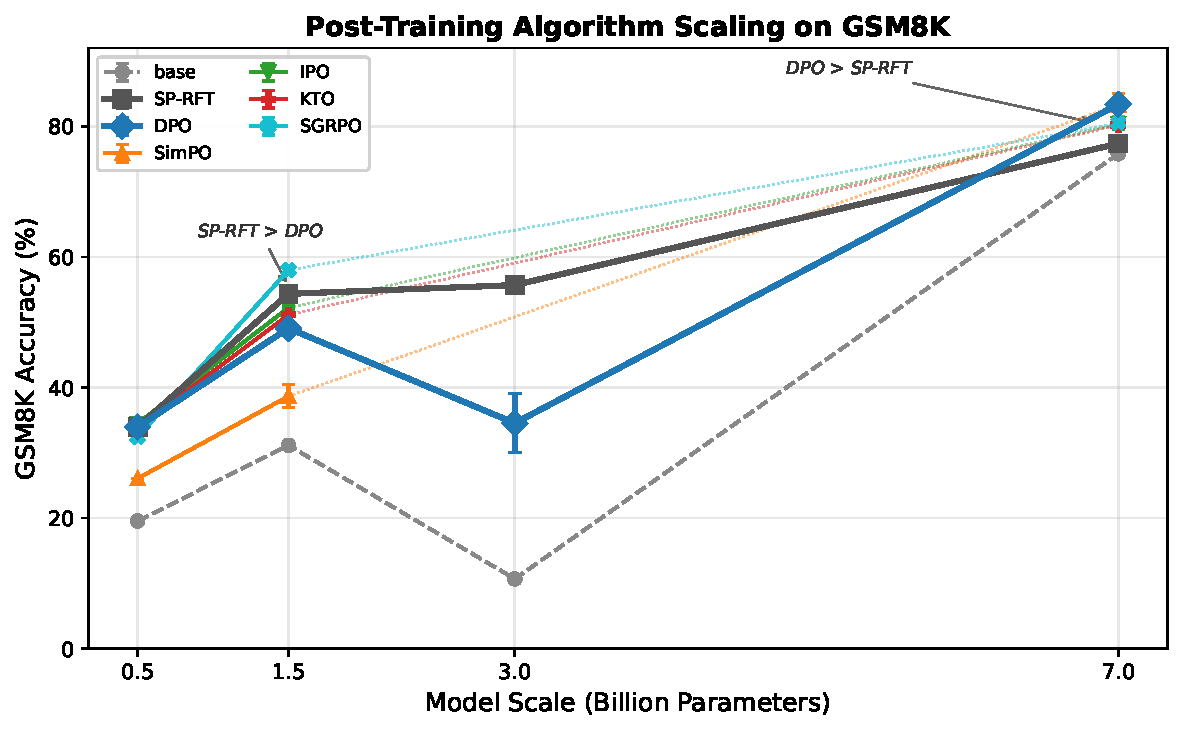
\includegraphics[width=0.8\textwidth]{scaling_curves_gsm8k.pdf}
\caption{GSM8K accuracy across model scales (Qwen 2.5). At 7B, no significant difference is detected between DPO and SimPO ($p = 0.95$, $N{=}5$), while \sprft{} separates by ${\sim}$6~pp ($p < 0.001$). The \sprft{}-to-preference \textbf{ranking inversion} between $\leq$3B and 7B is the paper's central finding.}
\label{fig:scaling_curves}
\end{figure}

\subsection{Cross-Architecture Validation and Deployment Scale}
\label{sec:cross_arch}

\textbf{Gemma 3 (1B--12B).} A natural objection is that the ranking inversion may be a Qwen-specific artifact.
To test generality, we train \sprft{}, DPO, and SimPO on Gemma~3 IT~\citep{gemma3_2025} at 1B, 4B, and 12B (3 seeds each, 27 runs). The pattern mirrors Qwen. At \textbf{1B}, \sprft{} dominates (26.7\%), DPO falls to 21.5\%, and SimPO collapses to 4.1\%. At \textbf{4B}, the same ordering holds with wider gaps: \sprft{} (75.3\%) $\gg$ DPO (57.8\%) $\gg$ SimPO (40.0\%). At \textbf{12B}---the critical test---DPO (87.4\%) overtakes \sprft{} (86.7\%), while SimPO (75.1\%) remains behind. This is the same \textbf{\sprft{}-to-DPO inversion} observed in Qwen: \sprft{} wins at small scale, DPO wins at large scale.

Two differences from Qwen are worth noting. First, SimPO does not converge to DPO at the largest scale in Gemma, suggesting that the DPO/SimPO parity observed at Qwen 7B may be architecture-specific. Second, the inversion point appears later in Gemma (12B vs.\ 7B), which may reflect differences in the pretrained model's formatting capabilities. Despite these nuances, the central finding---that \sprft{}-to-preference rankings invert with scale---replicates across architectures.

\textbf{Qwen 14B.} To extend the scaling curve beyond 12B, we train \sprft{}, DPO, and SimPO on Qwen~2.5-14B-Instruct with 3 seeds each (9 runs). The inversion persists: DPO (86.8\%~$\pm$0.23) $>$ SimPO (86.5\%~$\pm$0.68) $>$ \sprft{} (84.5\%~$\pm$0.19) $>$ Base (79.5\%). Within the Qwen family, the DPO--\sprft{} gap \emph{narrows} from 6.0~pp at 7B to \textbf{2.2~pp} at 14B, indicating that \sprft{} partially closes the gap at larger scale. On general benchmarks (ARC-C, HellaSwag, WinoGrande), the spread collapses to $<$1.2~pp, consistent with the format compliance finding.

Notably, MATH evaluation at 14B reveals a different pattern: SimPO (39.1\%) dramatically outperforms DPO (25.8\%) and \sprft{} (23.0\%), contrasting with Gemma~12B where DPO dominates MATH (50.2\% vs.\ SimPO 32.7\%). This architecture-dependent reversal on harder tasks further underscores that algorithm rankings cannot be extrapolated across models or tasks.

Table~\ref{tab:cross_arch} presents the combined cross-architecture and deployment-scale results.

\begin{table}[t]
\centering
\caption{Cross-architecture validation and deployment scale on GSM8K (\%). Gemma~3: 3 seeds each; 12B uses LoRA. Qwen~14B: 3 seeds each, LoRA. The \sprft{}-to-DPO inversion replicates across architectures and persists at 14B.}
\label{tab:cross_arch}
\small
\begin{tabular}{@{}lccccccc@{}}
\toprule
& \multicolumn{2}{c}{\textbf{Gemma 1B}} & \multicolumn{2}{c}{\textbf{Gemma 12B}} & \multicolumn{2}{c}{\textbf{Qwen 14B}} \\
\cmidrule(lr){2-3} \cmidrule(lr){4-5} \cmidrule(lr){6-7}
\textbf{Algorithm} & \textbf{Mean} & \textbf{$\pm\sigma$} & \textbf{Mean} & \textbf{$\pm\sigma$} & \textbf{Mean} & \textbf{$\pm\sigma$} \\
\midrule
\sprft{} & \textbf{26.7} & --- & 86.7 & 0.29 & 84.5 & 0.19 \\
DPO & 21.5 & --- & \textbf{87.4} & 0.26 & \textbf{86.8} & 0.23 \\
SimPO & 4.1 & --- & 75.1 & 4.88 & 86.5 & 0.68 \\
\midrule
\textit{\sprft{}$-$DPO gap} & \multicolumn{2}{c}{\textit{+5.2~pp}} & \multicolumn{2}{c}{\textit{$-$0.7~pp}} & \multicolumn{2}{c}{\textit{$-$2.2~pp}} \\
\bottomrule
\end{tabular}
\end{table}

\subsection{Finding 2: Initialization Dominates Algorithm Choice}
\label{sec:base_ablation}

Why do rankings invert? We hypothesize that algorithms interact differently with the prior alignment baked into Instruct checkpoints, and that removing this alignment should eliminate the differences.

Table~\ref{tab:base_ablation} tests this at 1.5B. Starting from Base, all methods improve (\sprft{}: +6.4~pp, DPO: +12.2~pp, SimPO: +23.2~pp) and the spread collapses from 15.7~pp to just \textbf{1.07~pp}.
SimPO---worst from Instruct---becomes best from Base, suggesting its reference-free nature makes it most sensitive to initialization.

Critically, this finding generalizes to 7B (Appendix~\ref{app:base_7b_ablation}): from Base, the spread collapses from 6.00~pp to 1.82~pp. The ranking from Base does \emph{not} simply reproduce the 1.5B pattern: at 1.5B Base, SimPO leads (61.87\%) followed by DPO (61.33\%) and \sprft{} (60.80\%); at 7B Base, \sprft{} leads (82.49\%) followed by SimPO (80.82\%) and DPO (80.67\%). Thus, a residual ranking shift persists even from Base---but the key observation is that these differences are compressed to $\leq$1.82~pp, compared to 6--16~pp from Instruct. Initialization is the dominant source of inter-algorithm variance, even if it does not fully explain it.

We note that DPO's sensitivity to Base initialization is theoretically expected: its KL regularization anchors the policy to the reference model, and a Base reference that cannot format math penalizes formatting improvements. However, the convergence extends to reference-free methods (SimPO) and pure \sprft{}, suggesting a more general phenomenon: the prior alignment state is the primary source of inter-algorithm variance, not just reference-model mechanics.
The practical significance is subtle: most real-world post-training starts from Instruct models, where algorithm choice \emph{does} produce measurable differences. But the Base ablations at both scales reveal that initialization explains most of these differences. Understanding the algorithm--initialization interaction appears more fruitful than designing new loss functions.

\begin{table}[t]
\centering
\caption{Base vs.\ Instruct initialization at 1.5B on GSM8K (\%). The spread collapses from 15.7~pp to 1.07~pp; SimPO reverses from worst to best. This compression generalizes to 7B (6.00~pp $\to$ 1.82~pp; Appendix~\ref{app:base_7b_ablation}).}
\label{tab:base_ablation}
\small
\begin{tabular}{@{}lccc@{}}
\toprule
\textbf{Algorithm} & \textbf{From Base} & \textbf{From Instruct} & \textbf{$\Delta$} \\
\midrule
\sprft{} & 60.80 & 54.36$_{\pm 0.59}$ & \textcolor{teal}{+6.4} \\
DPO & 61.33 & 49.08$_{\pm 0.61}$ & \textcolor{teal}{+12.2} \\
SimPO & \textbf{61.87} & 38.67$_{\pm 1.78}$ & \textcolor{teal}{+23.2} \\
\midrule
\textit{Spread} & \textit{1.07~pp} & \textit{15.7~pp} & \\
\bottomrule
\end{tabular}
\end{table}

\subsection{Finding 3: Two Regimes---Format Compliance, Then Architecture-Specific Reasoning}
\label{sec:format_compliance}

Tables~\ref{tab:math_results}~and~\ref{tab:math_scaling} compare GSM8K and MATH results. At 1.5B, the 19.3~pp GSM8K spread collapses to \textbf{0.54~pp} on MATH---a $36\times$ compression. Rankings shift: SGRPO drops from 1st to 4th, SimPO rises from last to 2nd. On general-domain benchmarks (ARC-C, HellaSwag, WinoGrande), the spread collapses further to \textbf{0.47~pp} ($41\times$; Appendix~\ref{app:figures}). At small scale, algorithms differ only in format compliance, not reasoning.

\textbf{But this picture changes at scale.} Table~\ref{tab:math_scaling} shows MATH accuracy across Gemma~3 scales. At 1B, the raw spread is 15.5~pp, but this is driven entirely by SimPO's catastrophic collapse to 1.1\%; excluding SimPO, Base/\sprft{}/DPO cluster within 2.9~pp. At 4B, DPO pulls ahead by +8.1~pp over \sprft{}. At 12B, DPO reaches 50.2\%---nearly \textbf{+9~pp over base and +17~pp over SimPO}. The spread among non-pathological methods \emph{increases} with scale, the opposite of the compression observed at 1.5B.

Critically, this pattern is \emph{architecture-dependent}. At Qwen~14B, \textbf{SimPO} dominates MATH (39.1\%~$\pm$2.2) over DPO (25.8\%~$\pm$0.4) by +13~pp---the reverse of Gemma. Meanwhile, general benchmarks (ARC-C, HellaSwag, WinoGrande; Appendix~\ref{app:general_benchmarks}) show $<$2~pp spread at all scales and both architectures. \textbf{Important caveat:} these are multiple-choice or perplexity-based benchmarks that evaluate log-likelihood ranking, not open-ended generation. Since post-training algorithms primarily alter the generative distribution, the absence of differences on MC benchmarks does not rule out inversions on generative tasks (e.g., AlpacaEval, MT-Bench). Our claim is narrower: the inversion is documented on mathematical reasoning; whether it extends to other \emph{generative} tasks remains open. The two-regime picture is: at small scale, algorithms differ shallowly (format); at large scale, algorithms differ deeply (reasoning), but \emph{which algorithm wins depends on architecture and task}. Both regimes make small-scale extrapolation unreliable.

\begin{table}[t]
\begin{minipage}[t]{0.48\textwidth}
\centering
\caption{Cross-task comparison at 1.5B: GSM8K vs.\ MATH. The 19.3~pp spread collapses to 0.54~pp ($36\times$ compression).}
\label{tab:math_results}
\small
\begin{tabular}{@{}lcc@{}}
\toprule
\textbf{Algorithm} & \textbf{MATH} & \textbf{GSM8K} \\
\midrule
\sprft{} & \textbf{27.04} & 54.36 \\
SimPO & 26.72 & 38.67 \\
KTO & 26.64 & 51.15 \\
SGRPO & 26.58 & \textbf{58.00} \\
DPO & 26.50 & 49.08 \\
\midrule
\textit{Spread} & \textit{0.54} & \textit{19.33} \\
\bottomrule
\end{tabular}
\end{minipage}
\hfill
\begin{minipage}[t]{0.50\textwidth}
\centering
\caption{MATH accuracy (\%) across scales. At $\geq$4B, DPO leads in Gemma but SimPO leads in Qwen~14B.}
\label{tab:math_scaling}
\small
\begin{tabular}{@{}lcccc@{}}
\toprule
& \multicolumn{3}{c}{\textbf{Gemma 3}} & \textbf{Qwen} \\
\cmidrule(lr){2-4} \cmidrule(lr){5-5}
& \textbf{1B} & \textbf{4B} & \textbf{12B} & \textbf{14B} \\
\midrule
Base & 16.6 & 34.4 & 41.3 & 16.8 \\
\sprft{} & 13.7 & 34.3 & 41.0 & 23.0 \\
DPO & 16.4 & \textbf{42.4} & \textbf{50.2} & 25.8 \\
SimPO & 1.1 & 39.2 & 32.7 & \textbf{39.1} \\
\bottomrule
\end{tabular}
\end{minipage}
\end{table}

\subsection{Controls: Disentangling Data Quality and RFT Artifacts}
\label{sec:controls}

\textbf{Fixed-dataset control.} Because self-play data is generated by each model, dataset quality correlates with model size---the most important confound in our design. To disentangle data quality from model scale, we train 1.5B Qwen~2.5 Instruct on self-play data generated by the \emph{14B} model---holding data quality fixed at the highest available level while keeping the learner at the scale where \sprft{} dominates. If the \sprft{}--DPO ranking at 1.5B were purely a data-quality artifact, providing 14B-quality data should flip the ranking in DPO's favor.

\textbf{\sprft{} still beats DPO by +5.1~pp} ($58.38\% \pm 0.49$ vs.\ $53.32\% \pm 0.70$, 3 seeds each), confirming that model scale---not data quality---is the primary driver of the ranking inversion. Both algorithms benefit comparably from higher-quality data (\sprft{}: +4.0~pp, DPO: +4.2~pp), leaving the gap stable (5.06~pp vs.\ 5.28~pp with own data).

\textbf{Gold-data SFT control.} Because \sprft{} trains on self-play trajectories (functionally RFT), a natural objection is that the ranking inversion merely reflects RFT's ceiling effect at scale, not a property of SFT \emph{per se}. To test this, we train standard SFT on MetaMathQA~\citep{yu2023metamath}---a high-quality, externally generated dataset of 240K GSM8K-related problems with expert solutions (3 seeds each at both 1.5B and 7B).

Tables~\ref{tab:fixed_dataset}--\ref{tab:gold_sft} report both controls side by side. At \textbf{1.5B}, Gold-SFT dominates all methods at $61.05\% \pm 0.45$, outperforming DPO by +12.0~pp. At \textbf{7B}, Gold-SFT reaches $83.32\% \pm 0.28$---\textbf{converging to DPO} ($83.38\% \pm 0.56$, gap: $-$0.06~pp). The SFT advantage collapses from +12~pp at 1.5B to statistical parity at 7B, regardless of whether the training data is self-generated or externally sourced. This \textbf{falsifies the RFT-artifact hypothesis}: even with high-quality gold data that eliminates the self-play ceiling, SFT's advantage over DPO still vanishes at scale.

\begin{table}[t]
\begin{minipage}[t]{0.46\textwidth}
\centering
\caption{Fixed-dataset control: 1.5B on \emph{14B} self-play data (GSM8K \%). \sprft{} still leads by +5.1~pp.}
\small
\begin{tabular}{@{}lcc@{}}
\toprule
\textbf{Algorithm} & \textbf{Mean} & $\sigma$ \\
\midrule
\sprft{} & \textbf{58.38} & 0.49 \\
DPO & 53.32 & 0.70 \\
\midrule
\textit{Gap} & \multicolumn{2}{c}{\textit{+5.06~pp}} \\
\bottomrule
\end{tabular}
\label{tab:fixed_dataset}
\end{minipage}
\hfill
\begin{minipage}[t]{0.52\textwidth}
\centering
\caption{Gold-SFT control: standard SFT on MetaMathQA (GSM8K \%). SFT advantage collapses from +12~pp to $\approx$0~pp with scale.}
\small
\begin{tabular}{@{}lcccc@{}}
\toprule
& \multicolumn{2}{c}{\textbf{1.5B}} & \multicolumn{2}{c}{\textbf{7B}} \\
\cmidrule(lr){2-3} \cmidrule(lr){4-5}
\textbf{Method} & \textbf{Mean} & $\sigma$ & \textbf{Mean} & $\sigma$ \\
\midrule
Gold-SFT & \textbf{61.05} & 0.45 & 83.32 & 0.28 \\
\sprft{} & 54.36 & 0.59 & 77.38 & 1.11 \\
DPO & 49.08 & 0.61 & \textbf{83.38} & 0.56 \\
\bottomrule
\end{tabular}
\label{tab:gold_sft}
\end{minipage}
\end{table}

\subsection{Practitioner Recommendations}
\label{sec:recommendations}

Our findings yield actionable guidance:
\begin{enumerate}[leftmargin=*,itemsep=1pt]
    \item \textbf{Validate at deployment scale, architecture, and task.} Rankings at $\leq$3B do not predict 7B+ behavior. Moreover, MATH rankings at Gemma~12B (DPO wins) reverse at Qwen~14B (SimPO wins). This is the paper's most important practical message.
    \item \textbf{DPO is a strong default on GSM8K.} DPO ranks near the top at both 1.5B and 7B in Qwen, overtakes \sprft{} at 12B in Gemma, and leads at 14B. It has the lowest seed variance ($\sigma = 0.56$ at 7B) and requires no special infrastructure. However, its advantage does not transfer uniformly to harder tasks (MATH).
    \item \textbf{Distrust variant sweeps at small scale.} The complete 1.5B$\to$7B ranking inversion among DPO variants means that small-scale variant selection is unreliable. Prefer vanilla DPO unless you can afford to validate at target scale.
    \item \textbf{Budget for multiple seeds at scale.} SimPO matches DPO in mean accuracy at 7B but with $3.2\times$ higher variance ($\sigma = 1.79$). Single-seed comparisons are misleading.
\end{enumerate}

% ================================================================
% 5. DISCUSSION
% ================================================================
\section{Discussion}
\label{sec:discussion}

\textbf{Why rankings invert: a mechanistic sketch.}
The Base-vs-Instruct ablation (Section~\ref{sec:base_ablation}) identifies one mechanism: ranking inversions arise partly from differential interaction between loss functions and prior alignment. We conjecture that at small scale, the Instruct model's limited capacity means that \sprft{}'s direct supervision provides the clearest gradient signal for format acquisition, while preference methods waste capacity modeling relative preferences between correct and incorrect solutions when the model can barely produce either. A complementary lens comes from viewing \sprft{} as RFT (Section~\ref{sec:methods}): at 1.5B, where the model rarely produces correct solutions, RFT on the few successful trajectories yields large gains precisely because the baseline is low. At 7B, the Instruct model already solves most GSM8K problems correctly, so RFT encounters a ceiling effect: training on filtered correct solutions offers diminishing returns, while DPO's contrastive signal---which leverages \emph{both} correct and incorrect trajectories---can still extract fine-grained reasoning improvements that teacher-forcing cannot provide. Critically, however, this RFT ceiling is \emph{not the whole story}: the gold-data SFT control (Section~\ref{sec:controls}) shows that even standard SFT on external expert data (MetaMathQA) converges to DPO at 7B ($83.32\%$ vs.\ $83.38\%$), despite dominating at 1.5B by +12~pp. The inversion is therefore not merely an artifact of self-play data saturation, but a genuine property of how supervised and contrastive objectives interact with model scale.

\textbf{What drives accuracy in mathematical reasoning.}
In decreasing order of leverage: model scale (${\sim}$50~pp), initialization (${\sim}$15~pp), training paradigm (\sprft{} vs.\ preference: ${\sim}$6~pp at 7B), and loss function choice within the preference family ($<$1~pp for DPO vs.\ SimPO on GSM8K; up to 5.8~pp across DPO variants at 7B).
On harder reasoning tasks (MATH), a new dimension emerges: algorithm-architecture interaction. DPO gains +9~pp on Gemma~12B MATH while SimPO gains +13~pp on Qwen~14B MATH---a complete reversal. This suggests that loss functions interact with architecture-specific representations in ways that are invisible on format-sensitive tasks like GSM8K.

\textbf{Methodological caveats at 7B+.}
Four design choices interact at 7B. (1)~The fixed LR ($10^{-6}$) is below the standard LoRA recommendation, but an ablation rules out under-training (Appendix~\ref{app:lr_ablation}). (2)~SGRPO was trained without explicit KL, but an ablation shows only +0.15~pp from adding it (Appendix~\ref{app:kl_ablation}). (3)~A 7B full-FT factorial (Appendix~\ref{app:lora_factorial}) confirms the inversion under both Full FT and LoRA, and the Gemma~3 replication plus 14B extension provide convergent evidence that scale is the primary driver. (4)~The effective batch size (8 prompts) is conservative relative to some DPO implementations (64--128). However, if small batches disproportionately hurt DPO through gradient variance, the inversion would be \emph{stronger} with larger batches---DPO already wins at 7B despite the small batch, making this a conservative design choice rather than one that inflates DPO's advantage. Online RL explorations (SGRPO, GSPO, CISPO) are reported in Appendix~\ref{app:online_rl}; the main paper focuses on offline methods where our coverage is most complete.

% ================================================================
% 6. CONCLUSION
% ================================================================
\section{Conclusion}

On mathematical reasoning, post-training algorithm rankings invert with scale: the method that wins at 1.5B loses at 7B, a finding replicated across Qwen~2.5 (up to 14B) and Gemma~3 (up to 12B) and confirmed with formal statistical testing ($p < 0.001$, $N{=}5$). On multiple-choice general benchmarks, algorithms differ by $<$1.2~pp at all scales---the inversion is task-specific within our evaluation suite. The inversion persists at 14B (DPO--\sprft{} gap of 2.2~pp), though the within-family gap narrows from 6.0~pp at 7B, suggesting \sprft{} partially closes the gap at larger scale. A fixed-dataset control confirms this is scale-driven: training 1.5B on 14B-quality data preserves the \sprft{}--DPO gap (5.1~pp vs.\ 5.3~pp with own data). Initialization---not the loss function---explains most algorithmic differences (3--15$\times$ spread compression when starting from Base). At small scale, residual differences largely reflect format compliance ($36\times$ spread compression from GSM8K to MATH at 1.5B), but at large scale MATH reveals genuine reasoning differences that are both architecture- and algorithm-dependent.

For mathematical reasoning, these results imply that the dominant paradigm---benchmarking algorithms at small scale and extrapolating to deployment---is unreliable and potentially counter-productive. Practitioners should validate at deployment scale. Whether this instability extends to other post-training objectives (instruction following, safety) is an important open question---our general-benchmark results suggest it may not, but those benchmarks are multiple-choice rather than generative, limiting their diagnostic power. The research community should invest in understanding how algorithms interact with scale, initialization, and task structure, rather than designing new loss functions evaluated at a single small scale.

\textbf{Limitations.}
Our study uses two model families (Qwen~2.5 up to 14B, Gemma~3 up to 12B) on mathematical reasoning. The ranking inversion is exclusively a mathematical reasoning phenomenon in our data: on general benchmarks (ARC-C, HellaSwag, WinoGrande), algorithms differ by $<$1.2~pp at all scales, with no observable inversion (Appendix~\ref{app:general_benchmarks}). However, these general benchmarks are multiple-choice or perplexity-based and do not test open-ended generation; generative instruction-following evaluations (e.g., AlpacaEval, MT-Bench) would provide a stronger test of whether the inversion extends beyond math. Generalization to instruction following, safety, or creative writing remains open. Because training data is self-generated at each scale, dataset quality covaries with model size. A fixed-dataset control at 1.5B and a gold-data SFT control at 1.5B and 7B jointly confirm that the inversion is not a data-source artifact; extending these controls to all scales would provide further evidence. The DPO variant sweep uses shared hyperparameters (LR, $\beta=0.1$) across all 20 variants; per-variant tuning could reveal differences that our plug-and-play protocol does not detect. All code, configs, and raw outputs are released for independent verification.\footnote{Code and data available upon acceptance.}

% ================================================================
% REFERENCES
% ================================================================
\begin{thebibliography}{30}

\bibitem[Azar et~al.(2024)]{azar2024general}
Azar, M.~G., Rowland, M., Piot, B., Guo, D., Calandriello, D., Valko, M., and Munos, R.
\newblock A general theoretical paradigm to understand learning from human feedback.
\newblock In \emph{International Conference on Artificial Intelligence and Statistics (AISTATS)}, 2024.

\bibitem[Chen et~al.(2024)]{chen2024spin}
Chen, Z., Deng, Y., Yuan, H., Ji, K., and Gu, Q.
\newblock Self-play fine-tuning converts weak language models to strong language models.
\newblock In \emph{International Conference on Machine Learning (ICML)}, 2024.

\bibitem[Cobbe et~al.(2021)]{cobbe2021gsm8k}
Cobbe, K., Kosaraju, V., Bavarian, M., Chen, M., Jun, H., Kaiser, L., Plappert, M., Tworek, J., Hilton, J., Nakano, R., Hesse, C., and Schulman, J.
\newblock Training verifiers to solve math word problems.
\newblock \emph{arXiv preprint arXiv:2110.14168}, 2021.

\bibitem[DeepSeek-AI(2025)]{deepseek2025r1}
DeepSeek-AI.
\newblock {DeepSeek-R1}: Incentivizing reasoning capability in {LLMs} via reinforcement learning.
\newblock \emph{arXiv preprint arXiv:2501.12948}, 2025.

\bibitem[Ethayarajh et~al.(2024)]{ethayarajh2024kto}
Ethayarajh, K., Xu, W., Muennighoff, N., Jurafsky, D., and Kiela, D.
\newblock {KTO}: Model alignment as prospect theoretic optimization.
\newblock In \emph{International Conference on Machine Learning (ICML)}, 2024.

\bibitem[Gao et~al.(2024)]{eval-harness}
Gao, L., Tow, J., Abbasi, B., Biderman, S., Black, S., DiPofi, A., Foster, C., Golding, L., Hsu, J., Le~Noac'h, A., Li, H., McDonell, K., Muennighoff, N., Ociepa, C., Phang, J., Reynolds, L., Schoelkopf, H., Skowron, A., Sutawika, L., Tang, E., Thite, A., Wang, B., Wang, K., and Zou, A.
\newblock The Language Model Evaluation Harness.
\newblock \url{https://github.com/EleutherAI/lm-evaluation-harness}, 2024.

\bibitem[Gemma Team(2025)]{gemma3_2025}
Gemma Team.
\newblock Gemma 3 technical report.
\newblock \emph{arXiv preprint arXiv:2503.19786}, 2025.

\bibitem[Hendrycks et~al.(2021)]{hendrycks2021math}
Hendrycks, D., Burns, C., Kadavath, S., Arora, A., Basart, S., Tang, E., Song, D., and Steinhardt, J.
\newblock Measuring mathematical problem solving with the {MATH} dataset.
\newblock In \emph{NeurIPS}, 2021.

\bibitem[Hong et~al.(2024)]{hong2024orpo}
Hong, J., Lee, N., and Thorne, J.
\newblock {ORPO}: Monolithic preference optimization without reference model.
\newblock In \emph{Conference on Empirical Methods in Natural Language Processing (EMNLP)}, 2024.

\bibitem[Hu et~al.(2022)]{hu2022lora}
Hu, E.~J., Shen, Y., Wallis, P., Allen-Zhu, Z., Li, Y., Wang, S., Wang, L., and Chen, W.
\newblock {LoRA}: Low-rank adaptation of large language models.
\newblock In \emph{ICLR}, 2022.

\bibitem[Ivison et~al.(2024)]{ivison2024unpacking}
Ivison, H., Wang, Y., Pyatkin, V., Lambert, N., Peters, M., Dasigi, P., Jang, J., Wadden, D., Smith, N.~A., Beltagy, I., and Hajishirzi, H.
\newblock Unpacking {DPO} and {PPO}: Disentangling best practices for learning from preferences.
\newblock In \emph{ACL Findings}, 2024.

\bibitem[Kwon et~al.(2023)]{kwon2023efficient}
Kwon, W., Li, Z., Zhuang, S., Sheng, Y., Zheng, L., Yu, C.~H., Gonzalez, J.~E., Zhang, H., and Stoica, I.
\newblock Efficient memory management for large language model serving with {PagedAttention}.
\newblock In \emph{ACM Symposium on Operating Systems Principles (SOSP)}, 2023.

\bibitem[Lucic et~al.(2018)]{lucic2018gans}
Lucic, M., Kurach, K., Michalski, M., Gelly, S., and Bousquet, O.
\newblock Are {GANs} created equal? {A} large-scale study.
\newblock In \emph{NeurIPS}, 2018.

\bibitem[Meng et~al.(2024)]{meng2024simpo}
Meng, Y., Xia, M., and Chen, D.
\newblock {SimPO}: Simple preference optimization with a reference-free reward.
\newblock In \emph{NeurIPS}, 2024.

\bibitem[Ouyang et~al.(2022)]{ouyang2022training}
Ouyang, L., Wu, J., Jiang, X., Almeida, D., Wainwright, C., Mishkin, P., Zhang, C., Agarwal, S., Slama, K., Ray, A., et~al.
\newblock Training language models to follow instructions with human feedback.
\newblock In \emph{NeurIPS}, 2022.

\bibitem[Qwen Team(2025)]{qwen2025qwen25}
Qwen Team.
\newblock {Qwen2.5} technical report.
\newblock \emph{arXiv preprint arXiv:2412.15115}, 2025.

\bibitem[Rafailov et~al.(2023)]{rafailov2023direct}
Rafailov, R., Sharma, A., Mitchell, E., Manning, C.~D., Ermon, S., and Finn, C.
\newblock Direct preference optimization: Your language model is secretly a reward model.
\newblock In \emph{NeurIPS}, 2023.

\bibitem[Rajbhandari et~al.(2020)]{rajbhandari2020zero}
Rajbhandari, S., Rasley, J., Ruwase, O., and He, Y.
\newblock {ZeRO}: Memory optimizations toward training trillion parameter models.
\newblock In \emph{International Conference on High Performance Computing, Networking, Storage and Analysis (SC)}, 2020.

\bibitem[Saeidi et~al.(2025)]{saeidi2025dpo_variants}
Saeidi, A., Verma, S., Uddin, M.~N., and Baral, C.
\newblock Insights into alignment: Evaluating {DPO} and its variants across multiple tasks.
\newblock In \emph{Proceedings of the 63rd Annual Meeting of the ACL: Student Research Workshop}, pages 409--421, 2025.

\bibitem[Schulman et~al.(2017)]{schulman2017proximal}
Schulman, J., Wolski, F., Dhariwal, P., Radford, A., and Klimov, O.
\newblock Proximal policy optimization algorithms.
\newblock \emph{arXiv preprint arXiv:1707.06347}, 2017.

\bibitem[Shao et~al.(2024)]{shao2024deepseekmath}
Shao, Z., Wang, P., Zhu, Q., Xu, R., Song, J., Zhang, M., Li, Y.~K., Wu, Y., and Guo, D.
\newblock {DeepSeekMath}: Pushing the limits of mathematical reasoning in open language models.
\newblock \emph{arXiv preprint arXiv:2402.03300}, 2024.

\bibitem[Spangher et~al.(2025)]{spangher2025rlhf}
Spangher, L., Pasumarthi, R.~K., Masiewicki, N., Arnold, W.~F., Kaushal, A., Johnson, D., Grabowski, P., and Ie, E.
\newblock {RLHF} algorithms ranked: An extensive evaluation across diverse tasks, rewards, and hyperparameters.
\newblock In \emph{Proceedings of the 2025 Conference on Empirical Methods in Natural Language Processing: Industry Track}, pages 518--529, 2025.

\bibitem[Tan et~al.(2025)]{tan2025rl_scaling}
Tan, Z., Geng, X., and 15 others.
\newblock Scaling behaviors of {LLM} reinforcement learning post-training: An empirical study in mathematical reasoning.
\newblock \emph{arXiv preprint arXiv:2509.25300}, 2025.

\bibitem[Touvron et~al.(2023)]{touvron2023llama2}
Touvron, H., Martin, L., Stone, K., Albert, P., Almahairi, A., Baber, Y., Bashlykov, N., Batra, S., Bhargava, P., Bhosale, S., et~al.
\newblock {Llama 2}: Open foundation and fine-tuned chat models.
\newblock \emph{arXiv preprint arXiv:2307.09288}, 2023.

\bibitem[Wu et~al.(2025)]{wu2025grpo_dpo}
Wu, Y., Ma, L., Ding, L., Li, M., Wang, X., Chen, K., Su, Z., Zhang, Z., Huang, C., Zhang, Y., Coates, M., and Nie, J.-Y.
\newblock It takes two: Your {GRPO} is secretly {DPO}.
\newblock \emph{arXiv preprint arXiv:2510.00977}, 2025.

\bibitem[Xu et~al.(2024)]{xu2024dpo}
Xu, S., Fu, W., Gao, J., Ye, W., Liu, W., Mei, Z., Wang, G., Yu, C., and Wu, Y.
\newblock Is {DPO} superior to {PPO} for {LLM} alignment? {A} comprehensive study.
\newblock In \emph{International Conference on Machine Learning (ICML)}, 2024.

\bibitem[Yu et~al.(2024)]{yu2023metamath}
Yu, L., Jiang, W., Shi, H., Yu, J., Liu, Z., Zhang, Y., Kwok, J.~T., Li, Z., Weller, A., and Liu, W.
\newblock {MetaMath}: Bootstrap your own mathematical questions for large language models.
\newblock In \emph{ICLR}, 2024.

\bibitem[Yuan et~al.(2023)]{yuan2023rft}
Yuan, Z., Yuan, H., Tan, C., Wang, W., Huang, S., and Huang, F.
\newblock Scaling relationship on learning mathematical reasoning with large language models.
\newblock \emph{arXiv preprint arXiv:2308.01825}, 2023.

\end{thebibliography}

% ================================================================
% APPENDIX
% ================================================================
\appendix

\section{Full DPO Variant Results}
\label{app:dpo_full}

\begin{table}[ht]
\centering
\caption{Taxonomy of 20 DPO variants evaluated in this study, organized by primary modification to the DPO objective. All evaluated at 1.5B on GSM8K with 5 seeds.}
\label{tab:dpo_taxonomy}
\small
\begin{tabular}{@{}llcc@{}}
\toprule
\textbf{Variant} & \textbf{Primary Modification} & \textbf{Ref.} & \textbf{Year} \\
\midrule
DPO & Baseline logistic loss & Y & 2023 \\
IPO & Squared loss regularization & Y & 2024 \\
SimPO & Length-normalized, no ref & N & 2024 \\
KTO & Unpaired binary feedback & Y & 2024 \\
Hinge & Hinge loss replacement & Y & 2024 \\
CPO & Contrastive preference & N & 2024 \\
ORPO & SFT-integrated preference & N & 2024 \\
RDPO & Robust divergence penalty & Y & 2024 \\
CDPO & Conservative DPO & Y & 2024 \\
BetaDPO & Adaptive $\beta$ scheduling & Y & 2024 \\
CalDPO & Calibrated reward margin & Y & 2024 \\
DPOP & Pref.-weighted optimization & Y & 2024 \\
ODPO & Online DPO & Y & 2024 \\
EXO & Exponentiated gradient & Y & 2024 \\
AlphaPO & Alpha-divergence pref. & N & 2024 \\
APO & Anchored preference & Y & 2024 \\
SPPO & Self-play preference & Y & 2024 \\
RobustDPO & Dist.\ robust DPO & Y & 2024 \\
GPO & Generalized pref.\ opt. & Y & 2024 \\
FocalPO & Focal loss preference & Y & 2024 \\
\bottomrule
\end{tabular}
\end{table}

\begin{table}[ht]
\centering
\caption{Full DPO variant results at 1.5B scale on GSM8K (5 seeds). $\Delta$ is the accuracy difference from vanilla DPO. $^\dagger$ indicates statistical significance after Bonferroni correction ($p < 0.0026$). Cohen's $d$ measures practical effect size.}
\label{tab:dpo_variant_full}
\small
\begin{tabular}{@{}llccccc@{}}
\toprule
\textbf{Variant} & \textbf{Category} & \textbf{Mean (\%)} & \textbf{Std} & \textbf{$\Delta$ DPO} & \textbf{$p$} & \textbf{$d$} \\
\midrule
ORPO & Reference-free & 53.89 & 0.60 & +4.12 & 0.0134 & 2.48 \\
DPOP & Weighting/calibration & 53.62 & 1.80 & +3.85 & 0.0189 & 1.88 \\
SPPO & Data augmentation & 52.60 & 1.45 & +2.84 & 0.0521 & 1.49 \\
IPO & Alternative divergence & 52.36 & 0.75 & +2.59 & 0.0614 & 1.53 \\
CalDPO & Weighting/calibration & 52.16 & 1.58 & +2.40 & 0.0934 & 1.22 \\
CPO & Reference-free & 51.43 & 1.57 & +1.67 & 0.2187 & 0.85 \\
GPO & Alternative divergence & 50.98 & 2.41 & +1.21 & 0.4370 & 0.52 \\
RobustDPO & Robustness & 50.89 & 2.13 & +1.12 & 0.4442 & 0.51 \\
CDPO & Robustness & 50.72 & 1.89 & +0.96 & 0.4916 & 0.46 \\
KTO & Unpaired & 50.48 & 2.11 & +0.71 & 0.6211 & 0.33 \\
Hinge & Alternative divergence & 49.87 & 2.43 & +0.11 & 0.9449 & 0.05 \\
DPO & Vanilla & 49.76 & 2.27 & -- & -- & -- \\
ODPO & Data augmentation & 48.37 & 3.20 & $-$1.39 & 0.4525 & $-$0.50 \\
APO & Data augmentation & 48.07 & 2.73 & $-$1.70 & 0.3175 & $-$0.68 \\
EXO & Data augmentation & 47.52 & 2.92 & $-$2.24 & 0.2145 & $-$0.86 \\
FocalPO & Weighting/calibration & 47.04 & 3.27 & $-$2.73 & 0.1686 & $-$0.97 \\
RDPO & Alternative divergence & 46.79 & 2.47 & $-$2.97 & 0.0835 & $-$1.25 \\
BetaDPO & Weighting/calibration & 45.75 & 4.31 & $-$4.02 & 0.1145 & $-$1.17 \\
AlphaPO & Reference-free & 41.68 & 5.13 & $-$8.08 & 0.0204 & $-$2.04 \\
SimPO$^\dagger$ & Reference-free & 38.23 & 2.12 & $-$11.54 & 0.0000 & $-$5.25 \\
\bottomrule
\end{tabular}
\end{table}

\textbf{Statistical notes.} Significance threshold: Bonferroni-corrected $\alpha = 0.05/19 = 0.0026$. Only SimPO ($p < 10^{-4}$) passes, and it is significantly \emph{worse}. ORPO ($p = 0.013$) and DPOP ($p = 0.019$) would be significant uncorrected but fail after correction. Our 5-seed design provides 80\% power to detect effects $\geq 1.0$~pp (Cohen's $d \geq 0.8$).

\textbf{At 7B: point-estimate rankings reverse.} We evaluate a stratified subset of 5 variants at 7B (3 seeds each), selected to span the 1.5B ranking (1st, 2nd, 7th, 13th, 15th). ORPO---1st at 1.5B---collapses to worst at 7B ($-$4.79~pp vs.\ DPO). EXO---15th at 1.5B---rises to the top ($+$1.00~pp). No variant reaches Bonferroni-corrected significance at either scale. The practical conclusion: since variant rankings are statistically unresolvable at both scales and their point estimates reverse, small-scale variant sweeps provide no reliable signal for large-scale behavior.

\textbf{Shared-hyperparameter design.} All 20 variants use the same LR ($10^{-6}$) and $\beta = 0.1$. This is a deliberate choice: the 20-variant sweep evaluates \emph{default-hyperparameter transferability}---whether variants provide gains ``out of the box'' with shared settings---not absolute algorithmic capability ceilings. This matches how practitioners typically deploy variants: using the original DPO paper's defaults. Per-variant tuning (e.g., optimizing $\beta$ for IPO's squared loss or KTO's unpaired feedback) could reveal differences that our shared-hyperparameter design masks. Our conclusion (variants are unresolvable) applies to the plug-and-play setting; per-variant tuning could surface real differences that shared hyperparameters mask.

\begin{table}[ht]
\centering
\caption{Stratified DPO variant evaluation at 7B (3 seeds each). Variants were selected to span the 1.5B ranking (1st, 2nd, 7th, 13th, 15th) to test rank-order predictiveness. Vanilla DPO: 83.38\% ($N{=}5$). Point-estimate rankings reverse: the 1.5B leader (ORPO) is the 7B laggard; the 1.5B underperformer (EXO) rises to top. No variant reaches Bonferroni-corrected significance at either scale.}
\label{tab:dpo_variant_7b}
\small
\begin{tabular}{@{}lccccc@{}}
\toprule
\textbf{Variant} & \textbf{Mean (\%)} & \textbf{Std} & \textbf{$\Delta$ DPO} & \textbf{$p$} & \textbf{1.5B Rank} \\
\midrule
EXO & \textbf{84.38} & 0.96 & $+$1.00 & 0.277 & 15th \\
ODPO & 83.88 & 1.31 & $+$0.49 & 0.654 & 13th \\
GPO & 83.40 & 1.05 & $+$0.02 & 0.984 & 7th \\
Vanilla DPO & 83.38 & 0.56 & --- & --- & 12th \\
DPOP & 80.92 & 1.18 & $-$2.46 & 0.085 & 2nd \\
ORPO & 78.59 & 1.04 & $-$4.79 & 0.013 & 1st \\
\bottomrule
\end{tabular}
\end{table}

\section{Training Configurations}
\label{app:configs}

\begin{table}[ht]
\centering
\caption{Shared training configuration across all experiments.}
\small
\begin{tabular}{@{}ll@{}}
\toprule
\textbf{Parameter} & \textbf{Value} \\
\midrule
Optimizer & AdamW ($\beta_1\!=\!0.9$, $\beta_2\!=\!0.95$, $\epsilon\!=\!10^{-8}$) \\
Weight decay & 0.01 \\
LR schedule & Cosine with 10\% linear warmup \\
Effective batch size & 8 prompts (1 $\times$ 8 grad.\ accum.) \\
Training epochs & 3 \\
Precision & BF16 mixed precision \\
Distributed strategy & DeepSpeed ZeRO Stage 3 \\
Hardware & $8\times$ NVIDIA H100 80GB HBM3 \\
Sequence length & 512 (math), 1024 (code) \\
\bottomrule
\end{tabular}
\end{table}

\begin{table}[ht]
\centering
\caption{Algorithm-specific hyperparameters.}
\small
\begin{tabular}{@{}llll@{}}
\toprule
\textbf{Algorithm} & \textbf{Learning Rate} & \textbf{Key Hyperparameters} & \textbf{GPUs/Run} \\
\midrule
\sprft{} & $1\!\times\!10^{-6}$ & -- & 1 \\
DPO & $1\!\times\!10^{-6}$ & $\beta = 0.1$ & 1 \\
SimPO & $1\!\times\!10^{-6}$ & $\beta = 0.1$, $\gamma = 0.5$ & 1 \\
IPO & $1\!\times\!10^{-6}$ & $\beta = 0.1$ & 1 \\
KTO & $1\!\times\!10^{-6}$ & $\beta = 0.1$ & 1 \\
SGRPO & $1\!\times\!10^{-6}$ & $\lambda_{\text{KL}} = 0$$^*$, $n = 4$ & 2 \\
GSPO & $1\!\times\!10^{-6}$ & $\lambda_{\text{KL}} = 0$, $n = 4$ & 2 \\
CISPO & $1\!\times\!10^{-6}$ & $\lambda_{\text{KL}} = 0$, $n = 4$, clip $= [0.8, 1.2]$ & 2 \\
\bottomrule
\end{tabular}
\vspace{2pt}
{\footnotesize $^*$Following the default GRPO recipe. See Appendix~\ref{app:kl_ablation} for an ablation with $\lambda_{\text{KL}} = 0.01$.}
\end{table}

For models at 7B/12B and for the 3B factorial, we apply LoRA~\citep{hu2022lora} with rank $r=16$, $\alpha=32$, applied to all linear layers. The core comparison at $\leq$3B/4B uses full fine-tuning.

\section{Framework Engineering}
\label{app:framework_eng}

Scaling online RL to 7B required resolving three critical infrastructure issues:
\textbf{(1)~Ray GPU over-subscription.} Fractional \texttt{num\_gpus} values in Ray caused GPU over-subscription deadlocks during multi-worker rollout generation; we enforce integer GPU allocation per worker.
\textbf{(2)~vLLM memory leak.} Rollout output objects were not explicitly freed between batches, causing a slow memory leak that triggered OOM after ${\sim}$200 steps at 7B; explicit deletion with \texttt{gc.collect()} resolved this.
\textbf{(3)~Epoch-transition OOM.} Optimizer state accumulated across epoch boundaries; offloading optimizer state to CPU between epochs eliminated the failure.

\section{LoRA Factorial}
\label{app:lora_factorial}

\begin{table}[ht]
\centering
\caption{2$\times$2 factorial disentangling scale from LoRA (Qwen 2.5). The inversion appears under both Full FT and LoRA at 7B: DPO (84.5\%) $>$ SimPO (83.6\%) $>$ \sprft{} (79.8\%) under Full FT, mirroring the LoRA ranking. 7B LoRA values: 5-seed means $\pm \sigma$; Full FT: single seed.}
\label{tab:lora_2x2}
\small
\begin{tabular}{@{}llcc@{}}
\toprule
& & \textbf{3B} & \textbf{7B} \\
\midrule
\multirow{4}{*}{\textbf{Full FT}} & Base & 10.69 & 75.82 \\
& \sprft{} & \textbf{18.35}$^b$ \small{(\textcolor{teal}{+7.7})} & 79.83 \small{(\textcolor{teal}{+4.0})} \\
& DPO & 14.44$_{\pm 2.01}$ \small{(\textcolor{teal}{+3.8})} & \textbf{84.46} \small{(\textcolor{teal}{+8.6})} \\
& SimPO & 6.90$^b$ \small{(\textcolor{red}{$-$3.8})} & 83.62 \small{(\textcolor{teal}{+7.8})} \\
\midrule
\multirow{4}{*}{\textbf{LoRA}} & Base & 10.69 & 75.82 \\
& \sprft{} & 18.04 \small{(\textcolor{teal}{+7.4})} & 77.38$_{\pm 1.11}$ \small{(\textcolor{teal}{+1.6})} \\
& DPO & 16.00 \small{(\textcolor{teal}{+5.3})} & \textbf{83.38}$_{\pm 0.56}$ \small{(\textcolor{teal}{+7.6})} \\
& SimPO & 6.90 \small{(\textcolor{red}{$-$3.8})} & 83.32$_{\pm 1.79}$ \small{(\textcolor{teal}{+7.5})} \\
\bottomrule
\end{tabular}
\end{table}

\section{Online RL Explorations}
\label{app:online_rl}

SGRPO (online RL) leads at 1.5B ($58.0\% \pm 0.57$, +3.6~pp over \sprft{}) at ${\sim}6\times$ the compute cost.
At 7B, SGRPO achieves 80.59\% (best of 3 epochs), placing it above \sprft{} but below DPO/SimPO. Adding KL regularization ($\lambda_{\text{KL}} = 0.01$) yields only +0.15~pp (Appendix~\ref{app:kl_ablation}), confirming that the online--offline gap is genuine rather than a regularization artifact. \textbf{Caveat:} SGRPO uses the same effective batch size (8 prompts) and fixed 3-epoch schedule as offline methods; online RL typically benefits from larger batches and dynamic rollout budgets, so our SGRPO results may underestimate online RL's true ceiling. SGRPO was not evaluated at 12B or 14B due to its ${\sim}6\times$ compute cost. Token-level SGRPO outperforms sentence-level GSPO by 12--18~pp; GSPO and CISPO results are below.\footnote{GSPO achieves 39.58\% at 1.5B; CISPO fails catastrophically (5.23\% at 1.5B, 0.15\% at 0.5B).}

\textbf{SGRPO at 3B.}
SGRPO at 3B achieves 4.93\% after epoch~1 and 8.11\% after epoch~2, both below the 10.69\% baseline. On-policy rollouts compound the format compliance crisis: poorly formatted generations receive no reward, preventing the policy from learning formatting.

\textbf{SGRPO at 7B.}
SGRPO achieves 80.59\% (best of 3 epochs; 80.59/80.29/79.91), above \sprft{} but below DPO/SimPO. Slight accuracy degradation at epochs 2--3 suggests overfitting to the reward signal.

\textbf{GSPO and CISPO.}
GSPO (sentence-level policy gradient) achieves 39.58\% at 1.5B and 19.86\% at 0.5B---12--18~pp below token-level SGRPO, demonstrating that credit assignment granularity is a high-impact choice within online RL.
CISPO fails catastrophically at all scales (0.15\% at 0.5B, 5.23\% at 1.5B).

\section{SimPO Variance Analysis}
\label{app:simpo_variance}

SimPO exhibits the highest seed variance of any method at any scale ($\sigma = 1.79$ at 7B vs.\ DPO's $\sigma = 0.56$). Across 5 seeds, SimPO's per-seed accuracy ranges from 81.50\% to 85.82\% (range: 4.32~pp), while DPO ranges from 82.79\% to 84.23\% (range: 1.44~pp)---a $3\times$ difference. SimPO's two highest and two lowest seeds cluster in pairs, consistent with a bifurcation in the optimization landscape. This bimodal pattern is absent in DPO. SimPO computes length-normalized log-probabilities without a reference model, lacking the implicit regularization of DPO's reference-anchored gradient. The practical consequence: SimPO's ``best seed'' appears to outperform DPO (85.82 vs.\ 84.23), but no significant difference is detected under proper multi-seed evaluation ($p = 0.95$).

\section{Additional Figures and Tables}
\label{app:figures}

\begin{table}[ht]
\centering
\caption{General-domain evaluation at 1.5B: ARC-Challenge (acc\_norm), HellaSwag (acc\_norm), WinoGrande (acc). The 19.3~pp GSM8K spread collapses to 0.47~pp ($41\times$ compression).}
\label{tab:general_domain_15b}
\small
\begin{tabular}{@{}lcccc@{}}
\toprule
\textbf{Algorithm} & \textbf{ARC-C (\%)} & \textbf{HellaSwag (\%)} & \textbf{WinoGrande (\%)} & \textbf{Avg (\%)} \\
\midrule
Base Model & 46.76 & 68.23 & 62.90 & 59.30 \\
\midrule
\sprft{} & 46.16 & 68.16 & 62.90 & 59.08 \\
DPO & 46.67 & 68.38 & 62.67 & 59.24 \\
IPO & 46.76 & 68.36 & 62.67 & 59.26 \\
KTO & \textbf{47.01} & 68.25 & 63.06 & 59.44 \\
SimPO & 46.08 & \textbf{68.37} & 62.59 & 59.01 \\
SGRPO & 46.67 & 68.23 & \textbf{63.54} & \textbf{59.48} \\
\midrule
\textit{Spread} & \textit{0.93} & \textit{0.22} & \textit{0.95} & \textit{0.47} \\
\bottomrule
\end{tabular}
\end{table}

\begin{table}[ht]
\centering
\caption{General-domain evaluation at 7B (LoRA). Despite a 6.0~pp GSM8K spread, the general-domain spread is just 0.71~pp.}
\label{tab:general_domain_7b}
\small
\begin{tabular}{@{}lcccc@{}}
\toprule
\textbf{Algorithm} & \textbf{ARC-C (\%)} & \textbf{HellaSwag (\%)} & \textbf{WinoGrande (\%)} & \textbf{Avg (\%)} \\
\midrule
Base Model & 55.20 & 80.48 & 71.11 & 68.93 \\
\midrule
\sprft{} & 55.29 \small{(\textcolor{teal}{+0.09})} & 80.45 \small{(\textcolor{red}{$-$0.03})} & 70.72 \small{(\textcolor{red}{$-$0.39})} & 68.82 \small{(\textcolor{red}{$-$0.11})} \\
DPO & 54.86 \small{(\textcolor{red}{$-$0.34})} & \textbf{80.58} \small{(\textcolor{teal}{+0.10})} & 70.72 \small{(\textcolor{red}{$-$0.39})} & 68.72 \small{(\textcolor{red}{$-$0.21})} \\
IPO & \textbf{55.55} \small{(\textcolor{teal}{+0.35})} & 80.37 \small{(\textcolor{red}{$-$0.11})} & \textbf{71.35} \small{(\textcolor{teal}{+0.24})} & \textbf{69.09} \small{(\textcolor{teal}{+0.16})} \\
KTO & 55.03 \small{(\textcolor{red}{$-$0.17})} & 80.39 \small{(\textcolor{red}{$-$0.09})} & 70.72 \small{(\textcolor{red}{$-$0.39})} & 68.71 \small{(\textcolor{red}{$-$0.22})} \\
SimPO & 54.44 \small{(\textcolor{red}{$-$0.77})} & 80.53 \small{(\textcolor{teal}{+0.05})} & 70.17 \small{(\textcolor{red}{$-$0.95})} & 68.38 \small{(\textcolor{red}{$-$0.56})} \\
\midrule
\textit{Spread (trained)} & \textit{1.11~pp} & \textit{0.21~pp} & \textit{1.18~pp} & \textit{0.71~pp} \\
\bottomrule
\end{tabular}
\end{table}

\begin{figure}[ht]
\centering
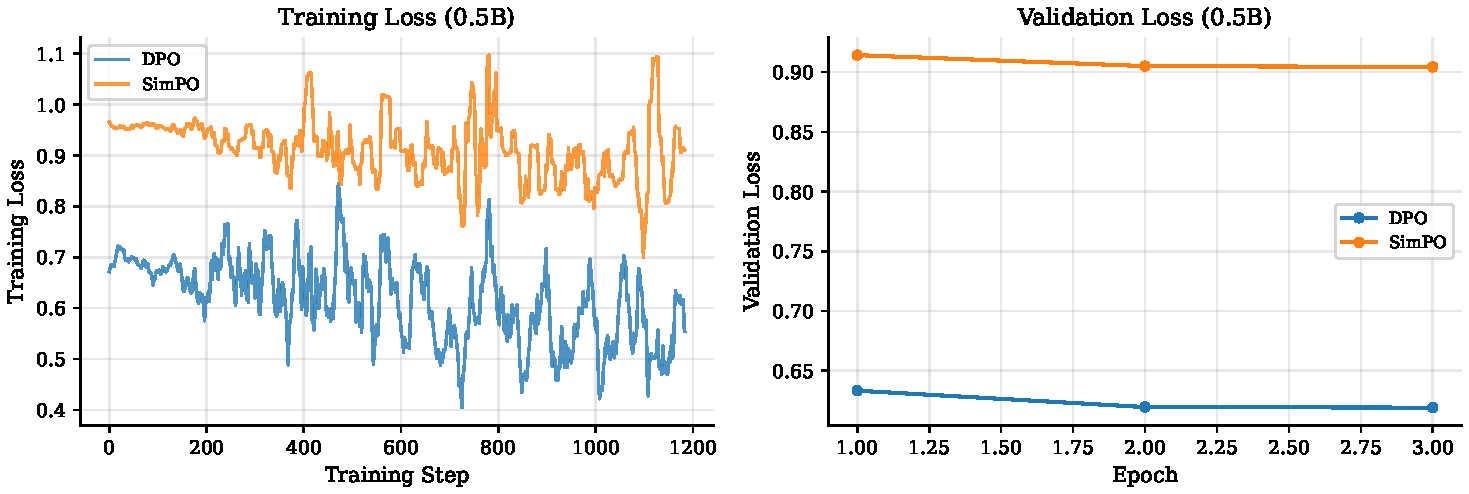
\includegraphics[width=\textwidth]{training_dynamics.pdf}
\caption{Training dynamics comparison at 0.5B scale. \textbf{Left:} training loss over steps (smoothed). \textbf{Right:} validation loss over epochs.}
\label{fig:training_curves_app}
\end{figure}

\begin{figure}[ht]
\centering
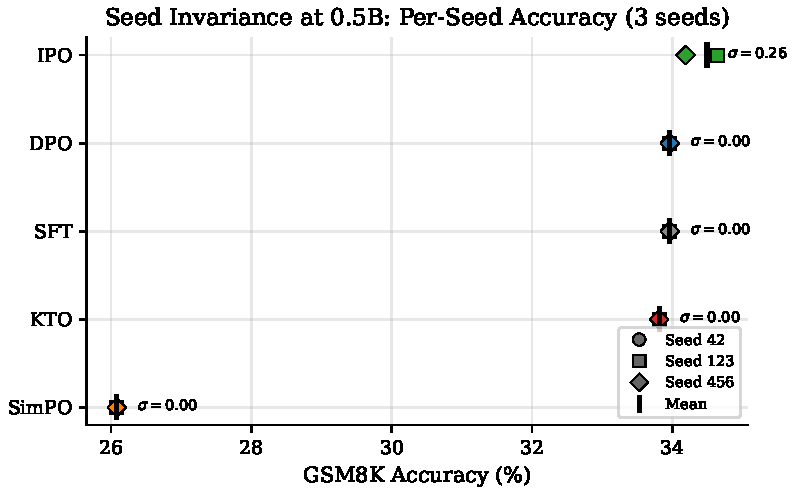
\includegraphics[width=0.75\textwidth]{seed_invariance_gsm8k.pdf}
\caption{Training determinism at 0.5B: per-seed GSM8K accuracy for each algorithm across 3 seeds. Five of six algorithms produce identical accuracy ($\sigma = 0$).}
\label{fig:seed_invariance_app}
\end{figure}

\section{Format Compliance Analysis}
\label{app:format}

Table~\ref{tab:format_gap} reports strict-match and flexible-extract accuracy. The \emph{format compliance gap} (strict $-$ flexible) quantifies whether a model produces well-formatted answers.

\begin{table}[ht]
\centering
\caption{Strict-match vs.\ flexible-extract accuracy on GSM8K. At 3B, the format compliance gap ranges from $-$26.2 to $-$33.7~pp across trained models, confirming format non-compliance drives the low strict-match scores.}
\label{tab:format_gap}
\small
\begin{tabular}{@{}llccr@{}}
\toprule
\textbf{Scale} & \textbf{Algorithm} & \textbf{Strict (\%)} & \textbf{Flexible (\%)} & \textbf{Gap (pp)} \\
\midrule
1.5B & \sprft{} & 54.66 & 55.57 & $-0.9$ \\
& DPO & 51.18 & 49.81 & $+1.4$ \\
& IPO & 52.39 & 52.31 & $+0.1$ \\
& KTO & 51.71 & 51.18 & $+0.5$ \\
& SimPO & 43.44 & 43.06 & $+0.4$ \\
\midrule
3B (full FT) & Base & 10.69 & 62.93 & $-52.2$ \\
 & \sprft{} & 18.04 & 44.28 & $-26.2$ \\
 & DPO & 16.45 & 42.91 & $-26.5$ \\
 & IPO & 16.83 & 45.72 & $-28.9$ \\
 & KTO & 15.31 & 44.50 & $-29.2$ \\
 & SimPO & 6.90 & 40.56 & $-33.7$ \\
\midrule
7B (LoRA) & \sprft{} & 76.42 & 80.29 & $-3.9$ \\
& DPO & 83.85 & 84.99 & $-1.1$ \\
& IPO & 81.35 & 83.09 & $-1.7$ \\
& KTO & 80.21 & 82.49 & $-2.3$ \\
& SimPO & 85.82 & 80.97 & $+4.9$ \\
\bottomrule
\end{tabular}
\end{table}

\section{Compute Budget}
\label{app:compute}

\begin{table}[ht]
\centering
\caption{Compute budget breakdown on H100 80GB GPUs.}
\label{tab:compute}
\small
\begin{tabular}{@{}lrrrr@{}}
\toprule
\textbf{Category} & \textbf{\# Runs} & \textbf{Time/Run} & \textbf{GPUs} & \textbf{GPU-h} \\
\midrule
Core 0.5B SL (5 algs $\times$ 3 seeds) & 15 & 4--8 min & 1 & 1.5 \\[2pt]
Core 0.5B RL (3 algs $\times$ 3 seeds) & 9 & $\sim$3 h & 2 & 54 \\[2pt]
Core 1.5B SL (5 algs $\times$ 3 seeds) & 15 & 14--27 min & 1 & 5.0 \\[2pt]
Core 3B SL full FT (3 algs) & 3 & 12--13 min & 1 & 0.6 \\[2pt]
3B LoRA factorial (3 algs) & 3 & 12--13 min & 1 & 0.6 \\[2pt]
Core 7B SL (5 algs $\times$ 1 seed) & 5 & 335--460 min & 1 & 30 \\[2pt]
Core 7B RL (SGRPO, 3 epochs) & 3 & $\sim$480 min & 2 & 48 \\[2pt]
7B multi-seed: \sprft{}/DPO/SimPO ($N{=}5$) & 13 & 330--360 min & 1 & 78 \\[2pt]
7B multi-seed: IPO/KTO ($N{=}3$) & 4 & 335--460 min & 1 & 27 \\[2pt]
MATH 1.5B evals (5 methods) & 5 & $\sim$30 min & 1 & 2.5 \\[2pt]
DPO variants 1.5B (20 $\times$ 5 seeds) & 100 & 14--27 min & 1 & 30 \\[2pt]
DPO variants 7B (5 $\times$ 3 seeds) & 15 & 330--360 min & 1 & 90 \\[2pt]
Ablations 1.5B & $\sim$57 & 9--10 min & 1 & 9 \\[2pt]
Ablations 7B (LR sweep, KL, Base init) & 16 & 330--480 min & 1--2 & $\sim$100 \\[2pt]
Gemma 3 (3 algs $\times$ 3 scales $\times$ 3 seeds) & 27 & varies & 1--2 & $\sim$75 \\[2pt]
7B Full FT factorial (\sprft{}/DPO/SimPO) & 3 & $\sim$180 min & 2 & 18 \\[2pt]
14B LoRA (\sprft{}/DPO/SimPO $\times$ 3 seeds) & 9 & $\sim$360 min & 2 & 108 \\[2pt]
Fixed-dataset control (\sprft{}/DPO $\times$ 3 seeds) & 6 & 14--27 min & 1 & 2.0 \\[2pt]
1.5B LR sweep (\sprft{}/DPO $\times$ 4 LRs $\times$ 3 seeds) & 18 & 14--27 min & 1 & $\sim$5.0 \\[2pt]
3B LR sweep (\sprft{}/DPO $\times$ 3 LRs $\times$ 3 seeds) & 18 & $\sim$25 min & 1 & $\sim$7.5 \\[2pt]
Gold-SFT control (1.5B $\times$ 3 + 7B $\times$ 3 seeds) & 6 & 27--360 min & 1 & $\sim$20 \\[2pt]
\midrule
\textbf{Total training} & $\sim$350 & -- & -- & $\sim$\textbf{720} \\[2pt]
Evaluation (GSM8K, MATH, general) & $\sim$430+ & 5--600 min & 1 & $\sim$220 \\[2pt]
\midrule
\textbf{Grand total} & & & & $\sim$\textbf{940 GPU-h} \\
\bottomrule
\end{tabular}
\end{table}

The total compute ($\sim$940 GPU-hours) is modest given the breadth ($\sim$350 training runs across 2 model families, 8 scales, 4 evaluation domains) and substantially less than training a single 7B model from scratch.

\section{Additional Scaling Results}
\label{app:scaling}

SGRPO at 1.5B achieves $58.00\% \pm 0.57$ (seeds: 57.47\%, 57.92\%, 58.61\%).
SL methods at 1.5B use multi-seed reruns with genuine variance (Table~\ref{tab:seedfix}).

\section{Multi-Seed Verification}
\label{app:seed_invariance}

\begin{table}[ht]
\centering
\caption{Multi-seed results at 1.5B on GSM8K (3 seeds each). Rankings preserved across seeds.}
\label{tab:seedfix}
\small
\begin{tabular}{@{}lcccccc@{}}
\toprule
\textbf{Method} & \textbf{Original} & \textbf{Mean} & \textbf{$\sigma$} & \textbf{s42} & \textbf{s123} & \textbf{s456} \\
\midrule
\sprft{} & 54.66 & 54.36 & 0.59 & 53.90 & 55.19 & 53.98 \\
IPO & 52.39 & 52.24 & 0.22 & 52.54 & 52.16 & 52.01 \\
KTO & 51.71 & 51.15 & 1.77 & 51.33 & 53.22 & 48.90 \\
DPO & 51.18 & 49.08 & 0.61 & 49.58 & 49.43 & 48.22 \\
SimPO & 43.44 & 38.67 & 1.78 & 36.85 & 38.06 & 41.09 \\
\bottomrule
\end{tabular}
\end{table}

\begin{table}[ht]
\centering
\caption{Multi-seed results at 7B (LoRA) on GSM8K. Core algorithms have $N{=}5$ seeds; IPO/KTO have $N{=}3$.}
\label{tab:seedfix_7b}
\small
\begin{tabular}{@{}lccccccccc@{}}
\toprule
\textbf{Method} & \textbf{$N$} & \textbf{Mean} & \textbf{$\sigma$} & \textbf{s42} & \textbf{s456} & \textbf{s789} & \textbf{s1024} & \textbf{s1337} \\
\midrule
DPO & 5 & \textbf{83.38} & 0.56 & 83.85 & 82.79 & 83.02 & 84.23 & 83.02 \\
SimPO & 5 & 83.32 & 1.79 & 85.82 & 81.50 & 82.64 & 85.06 & 81.58 \\
IPO & 3 & 80.39 & 0.92 & 81.35 & --- & 80.67 & --- & 79.15 \\
KTO & 3 & 80.24 & 0.16 & 80.21 & --- & 80.44 & --- & 80.06 \\
\sprft{} & 5 & 77.38 & 1.11 & 76.42 & 79.30 & 76.65 & 76.57 & 77.94 \\
\bottomrule
\end{tabular}
\end{table}

\textbf{Statistical tests at 7B.}
Welch's $t$-tests with Bonferroni correction ($\alpha = 0.05 / 10 = 0.005$):
\begin{itemize}[leftmargin=*,itemsep=1pt]
    \item \textbf{DPO vs.\ SimPO:} $\Delta = +0.06$~pp, $p = 0.950$. Not significant; no difference detected at this sample size.
    \item \textbf{DPO vs.\ \sprft{}:} $\Delta = +6.01$~pp, $p < 0.001$. \textbf{Significant.}
    \item \textbf{SimPO vs.\ \sprft{}:} $\Delta = +5.94$~pp, $p < 0.001$. \textbf{Significant.}
    \item \textbf{DPO vs.\ KTO:} $\Delta = +3.15$~pp, $p < 0.001$. \textbf{Significant.}
    \item \textbf{DPO vs.\ IPO:} $\Delta = +2.99$~pp, $p = 0.029$. Not significant after correction.
    \item \textbf{\sprft{} vs.\ IPO:} $\Delta = -3.01$~pp, $p = 0.018$. Not significant after correction.
    \item \textbf{\sprft{} vs.\ KTO:} $\Delta = -2.86$~pp, $p = 0.006$. Not significant after correction (marginal).
    \item \textbf{IPO vs.\ KTO:} $\Delta = +0.15$~pp, $p = 0.837$. Not significant.
\end{itemize}

Three groups emerge: (1) DPO/SimPO cluster (${\sim}$83.4\%), (2) IPO/KTO cluster (${\sim}$80.3\%), (3) \sprft{} (${\sim}$77.4\%). The DPO/SimPO $>$ \sprft{} separation is robust ($p < 0.001$).

\section{Sampling-Based Evaluation}
\label{app:sampling_eval}

We re-evaluate 1.5B and 7B checkpoints using nucleus sampling (top-$p = 0.9$, temperature $= 0.8$) with 8 samples per problem, reporting majority-vote accuracy.
Core rankings are preserved: at 7B, DPO and SimPO remain at the top, \sprft{} at the bottom. The inter-algorithm spread compresses slightly, consistent with sampling partially compensating for format compliance differences.

\section{Learning Rate Sensitivity at 7B}
\label{app:lr_ablation}

\begin{table}[ht]
\centering
\caption{Learning rate sensitivity for \sprft{} and DPO at 7B (LoRA) on GSM8K (\%). Each cell reports mean $\pm$ std over 3 seeds (\sprft{}) or 2 seeds (DPO). The default LR $= 10^{-6}$ is optimal for both algorithms; higher rates degrade performance monotonically.}
\label{tab:lr_ablation}
\small
\begin{tabular}{@{}lcccc@{}}
\toprule
\textbf{LR} & \textbf{\sprft{} Mean} & \textbf{\sprft{} Seeds} & \textbf{DPO Mean} & \textbf{DPO Seeds} \\
\midrule
$10^{-6}$ (default) & 77.38$_{\pm 1.11}$ & 5 seeds & 83.38$_{\pm 0.56}$ & 5 seeds \\
$5{\times}10^{-6}$ & 66.57$_{\pm 5.14}$ & 66.3 / 60.4 / 73.0 & 56.75$_{\pm 8.68}$ & 65.4 / 48.1 \\
$10^{-5}$ & 53.12$_{\pm 4.90}$ & 59.3 / 47.3 / 52.8 & 16.15$_{\pm 14.94}$ & 31.1 / \phantom{0}1.2 \\
$5{\times}10^{-5}$ & 30.20$_{\pm 7.73}$ & 34.1 / 37.1 / 19.4 & --- & --- \\
$2{\times}10^{-4}$ & \phantom{0}0.23 & 1 seed & --- & --- \\
\bottomrule
\end{tabular}
\end{table}

Three observations emerge. \textbf{(1)} The default $10^{-6}$ is optimal for both \sprft{} and DPO; no higher LR improves either algorithm, ruling out under-training as an explanation for \sprft{}'s 7B performance. \textbf{(2)} DPO is \emph{more} LR-sensitive than \sprft{}: at $10^{-5}$, DPO collapses to $16.15\%$ (one seed hits $1.2\%$) while \sprft{} retains $53.12\%$. \textbf{(3)} The ranking inversion (DPO $>$ \sprft{}) holds at the independently optimal LR for each algorithm ($10^{-6}$ for both), confirming it is not an artifact of hyperparameter tuning.

\textbf{Note on the lower boundary.} Our grid does not extend below $10^{-6}$ (e.g., to $5{\times}10^{-7}$). Because performance degrades \emph{monotonically and steeply} at every LR above $10^{-6}$---with DPO losing 27~pp at just $5{\times}$ higher---the gradient strongly favors the conservative end, and $10^{-6}$ already matches the recommended LoRA LR for both Qwen~2.5 and Gemma~3 in their official fine-tuning guides. Nonetheless, we cannot rule out a marginal improvement at $5{\times}10^{-7}$; if it exists, it would affect \sprft{} and DPO similarly and would not change the ranking inversion.

\section{Learning Rate Sensitivity at 1.5B}
\label{app:lr_ablation_15b}

To directly address whether the 1.5B \sprft{}--DPO ranking is an artifact of the shared LR ($10^{-6}$), we sweep LR in $\{5{\times}10^{-7}, 10^{-6}, 5{\times}10^{-6}, 10^{-5}\}$ for both \sprft{} and DPO at 1.5B with 3 seeds each (24 runs total).

\begin{table}[ht]
\centering
\caption{Learning rate sensitivity for \sprft{} and DPO at 1.5B (full FT) on GSM8K (\%). Each cell reports mean $\pm$ population std over 3 seeds. \sprft{} leads at \emph{every} LR. DPO collapses catastrophically at $\geq 5{\times}10^{-6}$. At independently optimal LRs, \sprft{}@$10^{-5}$ (56.61\%) beats DPO@$5{\times}10^{-7}$ (52.26\%) by +4.35~pp.}
\label{tab:lr_ablation_15b}
\small
\begin{tabular}{@{}lccccc@{}}
\toprule
\textbf{LR} & \textbf{\sprft{} Mean$_{\pm\sigma}$} & \textbf{\sprft{} Seeds} & \textbf{DPO Mean$_{\pm\sigma}$} & \textbf{DPO Seeds} \\
\midrule
$5{\times}10^{-7}$ & 53.83$_{\pm 0.21}$ & 54.13 / 53.68 / 53.68 & \textbf{52.26}$_{\pm 0.52}$ & 52.46 / 52.77 / 51.55 \\
$10^{-6}$ (default) & 54.36$_{\pm 0.59}$ & 55.19 / 53.90 / 53.98 & 49.08$_{\pm 0.61}$ & 49.43 / 49.58 / 48.22 \\
$5{\times}10^{-6}$ & 54.74$_{\pm 1.21}$ & 56.25 / 53.30 / 54.66 & 16.00$_{\pm 11.69}$ & 20.39 / 27.60 / \phantom{0}0.00$^\dagger$ \\
$10^{-5}$ & \textbf{56.61}$_{\pm 0.48}$ & 55.95 / 56.79 / 57.09 & 19.66$_{\pm 1.81}$ & 20.62 / 21.23 / 17.13 \\
\bottomrule
\multicolumn{5}{@{}l}{\footnotesize $^\dagger$Complete collapse: model generates only degenerate output.} \\
\end{tabular}
\end{table}

Four observations: \textbf{(1)} \sprft{} wins at every LR tested. \textbf{(2)} At independently optimal LRs, the gap widens to +4.35~pp. \textbf{(3)} DPO is dramatically more LR-sensitive at 1.5B than at 7B: the usable LR range for DPO shrinks from roughly one order of magnitude at 7B to half an order at 1.5B. \textbf{(4)} The 1.5B and 7B sweeps tell opposite stories about optimal LR, confirming that LR sensitivity itself is scale-dependent.

\section{Learning Rate Sensitivity at 3B}
\label{app:lr_ablation_3b}

The 3B collapse (Section~\ref{sec:ranking_inversion}) is fully recoverable with a LR sweep. We sweep LR in $\{5{\times}10^{-7}, 5{\times}10^{-6}, 10^{-5}\}$ for both \sprft{} and DPO at 3B (full FT) with 3 seeds each (18 runs).

\begin{table}[ht]
\centering
\caption{Learning rate sensitivity for \sprft{} and DPO at 3B (full FT) on GSM8K (\%). Each cell reports mean $\pm$ population std over 3 seeds. \sprft{} recovers to 55.7\% at $10^{-5}$---comparable to 1.5B Instruct---confirming the default-LR collapse was a hyperparameter pathology. \sprft{} leads at every LR.}
\label{tab:lr_ablation_3b}
\small
\begin{tabular}{@{}lccccc@{}}
\toprule
\textbf{LR} & \textbf{\sprft{} Mean$_{\pm\sigma}$} & \textbf{\sprft{} Seeds} & \textbf{DPO Mean$_{\pm\sigma}$} & \textbf{DPO Seeds} \\
\midrule
$5{\times}10^{-7}$ & 17.79$_{\pm 0.16}$ & 17.82 / 17.97 / 17.59 & 15.77$_{\pm 0.91}$ & 14.56 / 16.00 / 16.76 \\
$10^{-6}$ (default) & 18.35$^b$ & --- & 14.44$_{\pm 2.01}$ & 16.45 / 14.44 / 12.42 \\
$5{\times}10^{-6}$ & 41.80$_{\pm 3.84}$ & 40.26 / 38.06 / 47.08 & \textbf{34.55}$_{\pm 4.52}$ & 33.81 / 29.42 / 40.41 \\
$10^{-5}$ & \textbf{55.70}$_{\pm 1.09}$ & 54.21 / 56.79 / 56.10 & 16.30$_{\pm 7.34}$ & 5.91 / 21.46 / 21.53 \\
\bottomrule
\multicolumn{5}{@{}l}{\footnotesize $^b$Single seed from Table~\ref{tab:main_results}.} \\
\end{tabular}
\end{table}

Three observations: \textbf{(1)} The 3B collapse is fully recoverable for \sprft{}: at $10^{-5}$, it reaches 55.70\%---comparable to 1.5B Instruct (54.36\%). \textbf{(2)} \sprft{} wins at every LR, preserving the small-scale ranking. \textbf{(3)} DPO is dramatically more LR-sensitive than \sprft{} at 3B, mirroring the pattern at 1.5B and 7B.

\section{KL Regularization Ablation for SGRPO}
\label{app:kl_ablation}

\begin{table}[ht]
\centering
\caption{SGRPO at 7B with and without KL regularization on GSM8K (\%).}
\label{tab:kl_ablation}
\small
\begin{tabular}{@{}lccc@{}}
\toprule
\textbf{Method} & $\lambda_{\text{KL}}$ & \textbf{GSM8K (\%)} & \textbf{$\Delta$ vs.\ DPO} \\
\midrule
SGRPO (default) & 0 & 80.59 & $-$2.79 \\
SGRPO (regularized) & 0.01 & 80.74 & $-$2.64 \\
\midrule
DPO (reference) & $\beta = 0.1$ & 83.38$_{\pm 0.56}$ & --- \\
\bottomrule
\end{tabular}
\end{table}

Adding KL regularization yields only +0.15~pp, confirming the online--offline gap is genuine rather than a regularization artifact.

\section{Base vs.\ Instruct Initialization at 7B}
\label{app:base_7b_ablation}

\begin{table}[ht]
\centering
\caption{Base vs.\ Instruct initialization at 7B on GSM8K (\%). The spread collapses from 6.00~pp to 1.82~pp. \sprft{} leads from Base, reversing the Instruct ranking.}
\label{tab:base_7b_ablation}
\small
\begin{tabular}{@{}lccc@{}}
\toprule
\textbf{Algorithm} & \textbf{From Base (7B)} & \textbf{From Instruct (7B)} & \textbf{$\Delta$} \\
\midrule
\sprft{} & \textbf{82.49} & 77.38$_{\pm 1.11}$ & \textcolor{teal}{+5.11} \\
DPO & 80.67 & 83.38$_{\pm 0.56}$ & \textcolor{red}{$-$2.71} \\
SimPO & 80.82 & 83.32$_{\pm 1.79}$ & \textcolor{red}{$-$2.50} \\
\midrule
\textit{Spread} & \textit{1.82~pp} & \textit{6.00~pp} & \\
\bottomrule
\end{tabular}
\end{table}

From Base initialization at 7B, the ranking (\sprft{} $>$ SimPO $>$ DPO) differs from both the 1.5B Base ranking (SimPO $>$ DPO $>$ \sprft{}) and the 7B Instruct ranking (DPO $>$ SimPO $\gg$ \sprft{}). A residual ranking shift between scales persists even from Base, but at $\leq$1.82~pp---far smaller than the 6.00~pp Instruct spread. The key finding is that initialization accounts for the majority of inter-algorithm variance ($3.3\times$ compression at 7B, $14.7\times$ at 1.5B), even though a small scale-dependent residual remains.

\section{Hyperparameter Sensitivity}
\label{app:hp_sensitivity}

\begin{table}[ht]
\centering
\caption{$\beta$ sensitivity at 1.5B on GSM8K (\%). Both variants are stable across a $50\times$ range; default $\beta = 0.1$ is near-optimal.}
\label{tab:hp_sensitivity}
\small
\begin{tabular}{@{}lcccc@{}}
\toprule
\textbf{Variant} & $\beta = 0.01$ & $\beta = 0.1$ & $\beta = 0.5$ & \textbf{Range} \\
\midrule
DPOP & 54.66 & \textbf{55.19} & 53.30 & 1.89~pp \\
ORPO & 54.81 & 54.44 & 53.83 & 0.98~pp \\
\midrule
\textit{Vanilla DPO} & \multicolumn{3}{c}{\textit{49.76$_{\pm 2.27}$ (variant sweep)}} & \\
\bottomrule
\end{tabular}
\end{table}

\section{3B Flexible Extraction Analysis}
\label{app:3b_flex}

Under flexible extraction, the 3B base model achieves 62.93\%---comparable to the 1.5B Instruct model's strict-match performance. This reveals that the Qwen 2.5 3B Instruct model can \emph{solve} GSM8K problems at a competitive rate but fails to produce answers in the expected format. Post-training partially addresses this: \sprft{} reduces the format gap from $-$52.2~pp (base) to $-$26.2~pp.

\section{General Benchmark Results}
\label{app:general_benchmarks}

Table~\ref{tab:general_benchmarks} reports ARC-Challenge, HellaSwag, and WinoGrande accuracy across scales and architectures. At every scale and architecture, the spread is $<$2~pp---confirming that post-training algorithms do not meaningfully differ on these benchmarks. \textbf{This is a critical scope qualifier for our main findings:} the ranking inversion documented in this paper is specific to mathematical reasoning (GSM8K, MATH). On these general benchmarks, no inversion is observable, and algorithm choice is essentially irrelevant.

\textbf{Caveat: benchmark format.} ARC-C, HellaSwag, and WinoGrande are multiple-choice or perplexity-based evaluations, not open-ended generative tasks. Since our analysis identifies format compliance---a generative property---as the key differentiator at small scales (Section~\ref{sec:format_compliance}), the absence of algorithmic differences on non-generative benchmarks is expected and does not rule out the possibility that inversions occur on other \emph{generative} tasks. We leave this to future work.

\begin{table}[ht]
\centering
\caption{General benchmark accuracy (\%) after post-training. Spread remains $<$2~pp across all scales and architectures, confirming that algorithmic differences are task-specific.}
\label{tab:general_benchmarks}
\small
\begin{tabular}{@{}llcccc@{}}
\toprule
\textbf{Architecture} & \textbf{Algorithm} & \textbf{ARC-C} & \textbf{HellaSwag} & \textbf{WinoGrande} & \textbf{Avg} \\
\midrule
\multirow{4}{*}{Gemma 1B} & Base & 38.7 & 57.7 & 58.9 & 51.8 \\
& \sprft{} & 39.1 & 57.9 & 59.1 & 52.0 \\
& DPO & 38.7 & 57.6 & 58.8 & 51.7 \\
& SimPO & 39.6 & 57.2 & 57.6 & 51.5 \\
\midrule
\multirow{4}{*}{Gemma 12B} & Base & 61.1 & 81.9 & 74.6 & 72.5 \\
& \sprft{} & 60.1 & 81.7 & 74.5 & 72.1 \\
& DPO & 58.4 & 81.2 & 74.6 & 71.4 \\
& SimPO & 56.7 & 81.3 & 73.6 & 70.5 \\
\midrule
\multirow{4}{*}{Qwen 7B FT} & Base & 55.2 & 80.5 & 71.1 & 68.9 \\
& \sprft{} & 56.1 & 80.6 & 71.0 & 69.2 \\
& DPO & 55.0 & 80.6 & 70.4 & 68.7 \\
& SimPO & 54.1 & 80.6 & 69.9 & 68.2 \\
\midrule
\multirow{4}{*}{Qwen 14B} & Base & 62.4 & 84.4 & 76.0 & 74.3 \\
& \sprft{} & 61.9 & 84.5 & 75.2 & 73.9 \\
& DPO & 61.8 & 84.4 & 75.4 & 73.9 \\
& SimPO & 61.7 & 84.5 & 74.8 & 73.7 \\
\bottomrule
\end{tabular}
\end{table}

\end{document}
